\documentclass[sigconf]{acmart}

\usepackage{booktabs} % For formal tables
\usepackage{amsmath}
\usepackage[noend]{algpseudocode}
\usepackage[flushleft]{threeparttable}
\usepackage{subfigure}

\usepackage{comment}
\usepackage{color}
\usepackage{soul}
\usepackage{hyperref}
\usepackage{url}
\usepackage{multirow}

%\usepackage{algorithm}
%\usepackage[noend]{algpseudocode}
\usepackage[lined,linesnumbered,ruled]{algorithm2e}
\usepackage[flushleft]{threeparttable}
\usepackage{mfirstuc}

\def\sectionautorefname{Section}
\def\figureautorefname{Figure}
\def\subfigureautorefname{Figure}
\def\tableautorefname{Table}
\def\equationautorefname{Equation}

\makeatletter
\def\th@plain{%
  \thm@notefont{}% same as heading font
  \itshape % body font
}
\def\th@definition{%
  \thm@notefont{}% same as heading font
  % \normalfont % body font
	\itshape
}
\makeatother

\newtheorem{Def}{Definition}%[section]
%\def\definitionautorefname{Definition}
\newcommand{\Defautorefname}{Definition}

\newtheorem{Thm}{Theorem}%[section]
%\def\definitionautorefname{Definition}
\newcommand{\Thmautorefname}{Theorem}

%\newcommand{\Equautorefname}{Equation}

\def\on{{on}}
\def\off{{o\!f\!f}}
\def\dist{\mathrm{dist}}
\DeclareMathOperator{\tr}{tr}
\DeclareMathOperator{\proj}{proj}

%\renewcommand{\arraystretch}{1.5}

\newcommand{\ie}{i.e., }
\newcommand{\eg}{e.g., }
\newcommand{\note}[1]{\textbf{\color{blue}[***** #1 *****]\\}}
%\renewcommand{\note}[1]{}

% Problem specific macros
\newcommand{\probdef}{k-truss community search}
\newcommand{\Probdef}{K-truss community search}
\newcommand{\ProbDef}{\expandafter\capitalisewords\expandafter{\probdef}}
\newcommand{\inducedgraph}{induced MST graph}
\newcommand{\Inducedgraph}{Induced MST graph}
\newcommand{\InducedGraph}{\expandafter\capitalisewords\expandafter{\inducedgraph}}
\newcommand{\treeindex}{tree-structured community graph}
\newcommand{\Treeindex}{Tree-structured community graph}
\newcommand{\TreeIndex}{\expandafter\capitalisewords\expandafter{\treeindex}}


\newtheorem{case}{Use Case}

% Copyright
%\setcopyright{none}
%\setcopyright{acmcopyright}
%\setcopyright{acmlicensed}
\setcopyright{rightsretained}
%\setcopyright{usgov}
%\setcopyright{usgovmixed}
%\setcopyright{cagov}
%\setcopyright{cagovmixed}


%% DOI
%\acmDOI{10.475/123_4}
%
%% ISBN
%\acmISBN{123-4567-24-567/08/06}
%
%%Conference
%\acmConference[WOODSTOCK'97]{ACM Woodstock conference}{July 1997}{El
  %Paso, Texas USA} 
%\acmYear{1997}
%\copyrightyear{2016}
%
%\acmPrice{15.00}
%

%\newtheorem{theorem}{Theorem}

\begin{document}
\title{Fast Truss Community Query in Large-scale Dynamic Graphs}
%\titlenote{Produces the permission block, and
  %copyright information}
%\subtitle{Extended Abstract}
%\subtitlenote{The full version of the author's guide is available as
  %\texttt{acmart.pdf} document}


\author{Zheng Lu}
\affiliation{%
  \institution{University of Tennessee}
  \department{Electrical Engineering and Computer Science}
}
\email{zlu12@vols.utk.edu}

\author{Qing Cao}
\affiliation{%
  \institution{University of Tennessee}
  \department{Electrical Engineering and Computer Science}
}
\email{cao@utk.edu}

% The default list of authors is too long for headers}
\renewcommand{\shortauthors}{Z. Lu et al.}


\begin{abstract}
Recently, there has been significant interest in the study of the community search problem in social and information networks: given one or more query nodes, find densely connected communities containing the query nodes. However, most existing algorithms require linear computational time to the size of the found community for each specific K value. Therefore, state-of-the-art algorithms have limited scalability in large scale graphs, where communities grow to millions of edges.

In this paper, given an undirected graph G and a set of query
nodes $Q$, we study community query using the k-truss based community model. We formulate our problem of finding a connected truss community, as finding a connected k-truss subgraph with all possible k that contains Q. The state-of-art approximation algorithm can achieve this goal with a time complexity of $O(n'm')$ where $n'$ and $m'$ are the size of the result truss community. For queries that only identity and exact size of communities are required, We construct an index structure that can retrieve there information of all connected k-truss communities that contain $Q$ with all possible K values. The algorithm can run in $\sum_{u \in Q} d(u)$, where $d(u)$ is the degree of vertex $u$. We prove that this is the optimal time complexity for truss community query. Extensive experiments on real-world networks show the effectiveness and efficiency of our algorithms. 
\end{abstract}

%
% The code below should be generated by the tool at
% http://dl.acm.org/ccs.cfm
% Please copy and paste the code instead of the example below. 
%
%\begin{CCSXML}
%<ccs2012>
 %<concept>
  %<concept_id>10010520.10010553.10010562</concept_id>
  %<concept_desc>Computer systems organization~Embedded systems</concept_desc>
  %<concept_significance>500</concept_significance>
 %</concept>
 %<concept>
  %<concept_id>10010520.10010575.10010755</concept_id>
  %<concept_desc>Computer systems organization~Redundancy</concept_desc>
  %<concept_significance>300</concept_significance>
 %</concept>
 %<concept>
  %<concept_id>10010520.10010553.10010554</concept_id>
  %<concept_desc>Computer systems organization~Robotics</concept_desc>
  %<concept_significance>100</concept_significance>
 %</concept>
 %<concept>
  %<concept_id>10003033.10003083.10003095</concept_id>
  %<concept_desc>Networks~Network reliability</concept_desc>
  %<concept_significance>100</concept_significance>
 %</concept>
%</ccs2012>  
%\end{CCSXML}
%
%\ccsdesc[500]{Computer systems organization~Embedded systems}
%\ccsdesc[300]{Computer systems organization~Redundancy}
%\ccsdesc{Computer systems organization~Robotics}
%\ccsdesc[100]{Networks~Network reliability}

% We no longer use \terms command
%\terms{Theory}
%
%\keywords{ACM proceedings, \LaTeX, text tagging}


\maketitle

\section{Introduction}
\label{introduction}

Graphs are naturally used to model many real-world networks, \eg online social networks, biological networks, collaboration and communication networks. As community structures are commonly found in real-world networks, community related problems have been widely studied in the literature, such as community detection (\cite{newman2004finding, xie2013overlapping}) and community search (\cite{huang2014querying, akbas2017truss, huang2015approximate, lee2016query, sozio2010community, cui2014local, li2015influential, barbieri2015efficient}), and have found a wide range of applications (\cite{durmaz2017frequent,zong2015behavior,yin2017taming}). Triangles are known as fundamental building blocks of networks. K-truss as a definition of cohesive subgraph based on triangles of a graph, requires that each edge be contained in at least $(k - 2)$ triangles within this subgraph. The low computation cost of k-truss makes it suitable to scale to large-scale graphs.
The original definition of a k-truss lacks the connectivity constraint so that a k-truss may be an unconnected subgraph. \cite{huang2014querying} introduce the model of k-truss community based on triangle connectivity.

Community search, a query-dependent variant of community detection, attracts more attention as it enables targeted community discovery around given seed vertices of interest and is faster to process in the sense that the runtime does not depend on the size of the graph. However, all the relevant communities still have to be exhaustively identified, leading to excessive computation time/space if details of communities are not of interest. There are various types of queries that are useful in real-world applications involving communities that do not require details of communities. 
%The local community queries, such as community search, 
We can classify local community queries, such as community search, into two categories according to the level of information required to answer a query, the \toplevelprob{} query and the \bottomlevelprob{} query. The \toplevelprob{} query requires only relation information between different communities of interest. For example, "Do query vertices belongs to the same communities?", "What is the level of cohesiveness among all query vertices?". It is possible to process this type of queries by only examining relations between relavant communities to which query vertices belong without diving into inside structures of them. Another type of queries, the \bottomlevelprob{} query, requires edge level information to process, for example, the widely studied community search problem or finding boundaries of a target community. One has to know edge level structures inside relevant communities to be able to answer such queries.

\begin{figure}[ht]
    \centering
    \includegraphics[width=0.8\linewidth]{./figures/illustration_main.png}
    \caption{Two layer index structure for k-truss community queries.}
    \label{fig:illustration_main}
		\vspace{-0.2 in}
\end{figure}

Local community queries, such as community search, based on the k-truss community model (\cite{huang2014querying}) can benefit from compact index structures constructed from pre-computed results due to the low computational cost of the k-truss community model. Previous works mainly focused on community search problem of a single query vertex (\cite{huang2014querying, akbas2017truss}). In this paper, we propose a novel 2-level index structure, to support both the \toplevelprob{} and the \bottomlevelprob{} k-truss community query. An overview of our \twolevelindex{} is shown in \autoref{fig:illustration_main}. The top level index is a super-graph with vertices represent unique k-truss communities and edges represent containment relations between k-truss communities. For the bottom level index, We introduce a new type of graph called triangle derived graph that translates triangle connectivity in a graph to edge connectivity for fast k-truss community traversal. We store a maximum spanning forest of the triangle derived graph generated from the underlying graph that preserves the detailed edge level structure of k-truss communities in the bottom level index. 
%We combine the top level index and bottom level index together by partition the bottom level index based on 
%We partitioned this maximum spanning tree according to k-truss communities and the subgraph belonging to each k-truss community separatel. 
The super-graph forms a forest, and we can use simple $union$ and $intersection$ operations to locate relevant k-truss communities of a given query. 
To handle local k-truss community queries, we can use simple $union$ and $intersection$ operations on the top level index to efficiently locate target communities of a query. These communities can be used to answer \toplevelprob{} queries directly or handed to the bottom level index to processing inner-community details for \bottomlevelprob{} queries. The bottom level index is only used for \bottomlevelprob{} queries that using edge level information to further process relevant communities provided by the top level index. For example, in a community search query, we can first use the top level index to find target k-truss communities that contain all query vertices and then use the bottom level index to retrieve edges contained in each target k-truss community. The \twolevelindex{} proposed in this paper can efficiently process both single-vertex queries and multiple-vertex queries. We proved our index and query process to be theoretically optimal and showed its efficiency in practice for both \toplevelprob{} and \bottomlevelprob{} k-truss community queries on real-world graphs and demonstrate its performance by comparing with state-of-the-art methods, the TCP index (\cite{huang2014querying}) and the Equitruss index (\cite{akbas2017truss}). For reproducibility, we make the source code available online.\footnote{https://github.com/DongCiLu/KTruss1 34}

Our contribution can be summarized as follows.
\begin{itemize}
	\item We categorize the local k-truss community queries into the \toplevelprob{} query and the \bottomlevelprob{} query based on the information required to answer each type of query. 
	%which is supported by various query types. The k-truss community identity search is efficient for many real-world applications and is much more efficient than k-truss community search based approach.
	\item We develop a 2-level index structure that can efficiently process both the \toplevelprob{} and the \bottomlevelprob{} k-truss community query. The top level index contains a super-graph for locating target communities of a given query. The bottom level index preserves the edge level triangle connectivity for detailed search of inner-community structures.  
	%\item We design an efficient bottom-up index construction algorithm for our 2-level index structure. The time and space complexity is $O(m\log{m})$ and $O(m)$ respectively.
	\item We perform extensive experiments on our 2-level index on large-scale real-world graphs and compare it with state-of-the-art index structures. We can process \toplevelprob{} queries in the range of hundreds of microseconds to less than a second. We can process \bottomlevelprob{} queries in the range of few seconds to hundreds of seconds for highest degree vertices within large communities. %Our index The results show that our index is not only much compact and efficient for k-truss community search queries but can also support various query types.
\end{itemize}

The rest of this paper is organized as follows. Section~\ref{preliminary} provides notations and definitions used in this paper. We design a novel 2-level index structure in Section~\ref{index}. Section~\ref{query} discusses the query process on the proposed index structure. The evaluations of our algorithm are in Section~\ref{evaluation}.  We discuss previous works in Section~\ref{relatedwork} and conclude our work in Section~\ref{conclusion}.


\section{Preliminaries}
\label{preliminary}

\begin{figure}[ht]
    \centering
    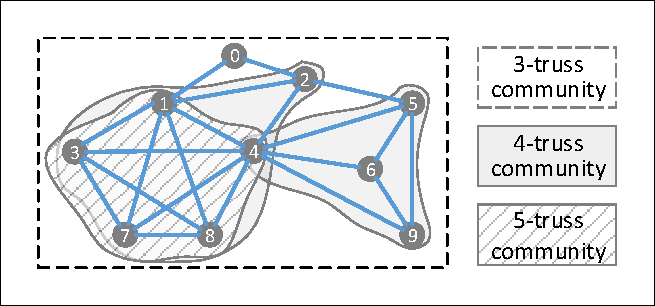
\includegraphics[width=0.7\linewidth, trim={0.6cm 0.6cm, 0.6cm, 0.6cm}, clip]{./figures/k-truss.pdf}
		\vspace{-0.2cm}
    \caption{An example graph with four k-truss communities}
    \label{fig:example}
		\vspace{-0.2cm}
\end{figure}

In our problem, we consider an undirected graph $G = (V,E)$. An example graph is shown in \autoref{fig:example}.
%The number of vertices is denoted as $n = |V|$ and number of edges is denoted as $m = |E|$. 
%We use $w_u$ and $w_e$ to denote the weight of a vertex $u$ and an edge $e$. 
We define the set of neighbors of a vertex $v$ in $G$ as $N_v = {u \in V :(v, u) \in E}$. %and the degree of $v$ as $d_v = |N_v|$. %We define a triangle $\triangle_{uvw}$ as a cycle of length $3$ with distinct vertices $u, v, w \in V$. 
We follow definitions of basic concepts used in \cite{huang2014querying}. The support of an edge $e_{u,v} \in E$ is defined as the number of triangles an edge belongs to and denoted as $s_{e,G}$. 

%\begin{Def}[Edge support]
%The support of an edge $e_{u,v} \in E$ is defined as $s_{e,G} = |{\triangle_{uvw} : w \in V}|$. 
%%We denote it as $s_e$ when the context is clear.
%\label{def:edge_support}
%\end{Def}

%For example, in \autoref{fig:example}, the edge support for $(0,2)$ is $2$, as it is contained in triangle $(0,2,1)$ and triangle $(0,2,4)$.

\begin{Def}[Trussness] 
The trussness of a subgraph $G^{\prime} \in G$ is the minimum support of edges in $G^{\prime}$ plus $2$, denoted by $\tau_{G^{\prime}}$. Edge trussness is defined as $\tau_{e} = max_{G^{\prime} \in G}\{\tau_{G^{\prime}}: e \in E_{G^{\prime}}\}$.
\label{def:trussness}
\end{Def}

For example, in \autoref{fig:example}, subgraph $(1,3,7,8,4)$ has trussness of $5$ as all edges in it have support at least $5-2=3$. The trussness of edge $(1,4)$ is also $5$.

\begin{Def}[k-truss]
Given a graph $G$ and $k \ge 2$, $G^{\prime} \subseteq G$ is a k-truss if $\forall e \in E_{G^{\prime}}, s_{e,G^{\prime}} \ge (k - 2)$. 
$G^{\prime}$ is a maximal k-truss if it is not a subgraph of another k-truss subgraph with the same trussness $k$ in $G$.
\label{def:k-truss}
\end{Def}

%\begin{Def}[Maximal k-truss subgraph]
%$H$ is a maximal k-truss subgraph if it is not a subgraph of another k-truss subgraph with same trussness $k$ in $G$.
%\label{def:maximal_k-truss}
%\end{Def}

%Because the K-truss definition does not define the connectivity, we use the definition of triangle connectivity used in \cite{huang2014querying}. 
Two triangles are adjacent if they share a common edge. Two edges are triangle connected if they belongs to the same triangle or they can reach each other through a series of adjacent triangles. %For example, in \autoref{fig:example}, $(1,4)$ is triangle connected to $(5,6)$ through a series of adjacent triangles $(1,2,4)$, $(2,4,5)$ and $(4,5,6)$.
%
%\begin{Def}[Triangle adjacency]
%${\triangle}_{1}$, ${\triangle}_{2}$ are adjacent if they share a common edge, i.e., ${\triangle}_{1} \cap {\triangle}_{2} \neq \emptyset$. 
%\label{def:triangle_adjacency}
%\end{Def}

%\begin{Def}[Triangle connectivity] 
%${\triangle}_{1}$, ${\triangle}_{2}$ are triangle connected if they can reach each other through a series of adjacent triangles, \ie for $1 \le i < n, {\triangle}_{i} \cap {\triangle}_{i-1} \neq \emptyset$. Two edges $e_1$, $e_2$ are triangle connected if $\exists e_{1} \in {\triangle}_{1}$, $e_{2} \in {\triangle}_{2}$, ${\triangle}_{1}$ and ${\triangle}_{2}$ are identical or triangle connected.
%\label{def:triangle_connectivity}
%\end{Def}

\begin{figure*}[ht]
    \centering
    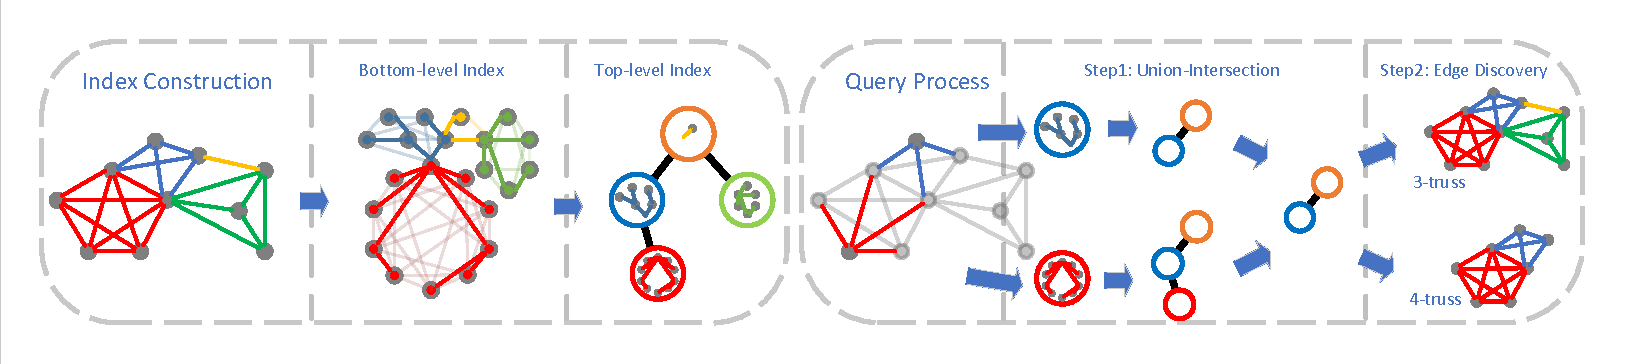
\includegraphics[width=0.9\linewidth, trim={0.6cm 0.6cm, 0.6cm, 0.6cm}, clip]{./figures/flow.pdf}
		\vspace{-0.2cm}
    \caption{Index construction and Query process on \twolevelindex{}}
    \label{fig:flow}
		\vspace{-0.5cm}
\end{figure*}

%\begin{Def}[Triangle connected graph]
%Two edge $e_{1}, e_{2}$ are triangle connected in a subgraph $H$ if there are two triangle ${\triangle}_{1}, {\triangle}_{2}$ in $H$ and $e_{1} \in {\triangle}_{1}, e_{2} \in {\triangle}_{2}$, either ${\triangle}_{1} = {\triangle}_{2}$, or ${\triangle}_{1}$ is triangle connected with ${\triangle}_{2}$ in $H$.
%A graph $G$ is triangle connected if all pairs of edges in $G$ are triangle connected.
%\label{def:triangle_connected_graph}
%\end{Def}

Finally, we define k-truss community based on the definition of k-truss subgraph and triangle connectivity as follows.

\begin{Def}[K-truss community] 
A k-truss community is a maximal k-truss with all its edges triangle connected.
\label{def:k-truss_community}
\end{Def}

\autoref{fig:example} shows several examples of k-truss communities. The whole example graph is a $3$-truss community as every edge has the support of at least $1$ and all edges are triangle connected. Note that there are two separate $4$-truss communities. Because $(2,5)$ has the support of $1$, it cannot belong to a $4$-truss. After excluding edge $(2,5)$, edges in the two $4$-trusses are no longer triangle connected.
%The problem studied in this paper is to build index structures to answer K-truss community related queries.
%defined as follows. Given a graph $G(V,E)$, a set of query vertices $Q \in V$, find all truss communities containing $Q$ with maximum $k$, a specific $k$ or any possible $k$. 
\section{\TwoLevelIndex{}}
\label{index}

In this paper, we aim to solve \probdef{} problems with a novel \twolevelindex{}. We describe the structure and construction of the \twolevelindex{} in this section. Then We show how to use the \twolevelindex{} to process various kinds of k-truss community queries in the next section.

%\subsection{Overview}
The index proposed in this paper contains two levels. The top level index provides information at the community level while the bottom level index offers information at the edge level. The top level is a super-graph, called \treeindex{}, whose vertices represent unique k-truss communities and edges represent containment relations between k-truss communities. The bottom level is a maximum spanning forest of a \inducedgraph{} that preserves the edge level trussness and triangle connectivity inside k-truss communities. An overview of the index is shown in \autoref{fig:illustration_main}. 

The index is constructed in a bottom-up manner. In the following, we first formally define the \inducedgraph{} and introduce the algorithm of constructing it from the original graph (Section~\ref{bottom-level}). Then we introduce the \treeindex{} and show how to use simple graph traversals on the \inducedgraph{} to create the \treeindex{} (Section~\ref{top-level}). Finally, we show the structure we used for the \twolevelindex{} to combine the \inducedgraph{} and the \treeindex{} (Section~\ref{structure}).

\subsection{\InducedGraph{}}
\label{bottom-level}
%\usernote{use counting sort}
The \inducedgraph{} of an original graph $G^o$ is obtained by associating a vertex with each edge of $G^o$ and connecting two vertices if the corresponding edges of $G^o$ belong to the same triangle. Then we only store a maximum spanning tree of the \inducedgraph{} to save edge level structures of k-truss communities in the original graph. By using a maximum spanning forest of the \inducedgraph{} as the bottom level index, we can use minimum edge enumerations to replace computational expensive triangle enumerations at query time. We show the formal definition of the \inducedgraph{} in \autoref{def:\inducedgraph{}}.

\begin{Def}[\Inducedgraph{}]
The \inducedgraph{} $G^t$ is a weighted undirected graph that each edge in the original graph $G^o$ is represented as a vertex in $G^t$. $G^t$ has an edge $e^{t}$ connecting vertices $v^{t}_{1}, v^{t}_{2} \in G^{t}$ if and only if their corresponding edges $e^{o}_{1}, e^{o}_{2} \in G^{o}$ belong to the same triangle in $G^o$. The weight of a vertex in $G^{t}$ is the trussness of its corresponding edge in $G^o$. The weight of an edge in $G^{t}$ is the lowest trussness of edges in the corresponding triangle in $G^{o}$. 
\label{def:\inducedgraph{}}
\end{Def}

We show an example of the \inducedgraph{} and a maximum spanning forest of it in \autoref{fig:\inducedgraph{}}. We outline the maximum spanning forest in \autoref{fig:example} with bold lines. %The rest lines are edges that are generated by \autoref{alg:\inducedgraph{}_construction} but discarded by the algorithm when generate the maximum spanning tree. 

%\begin{Def}[\inducedgraph{}]
%The \inducedgraph{} $G^m$ is a maximum spanning forest of the transformed graph $G^t$.
%\label{def:\inducedgraph{}}
%\end{Def}

\begin{figure}[ht]
    \centering
    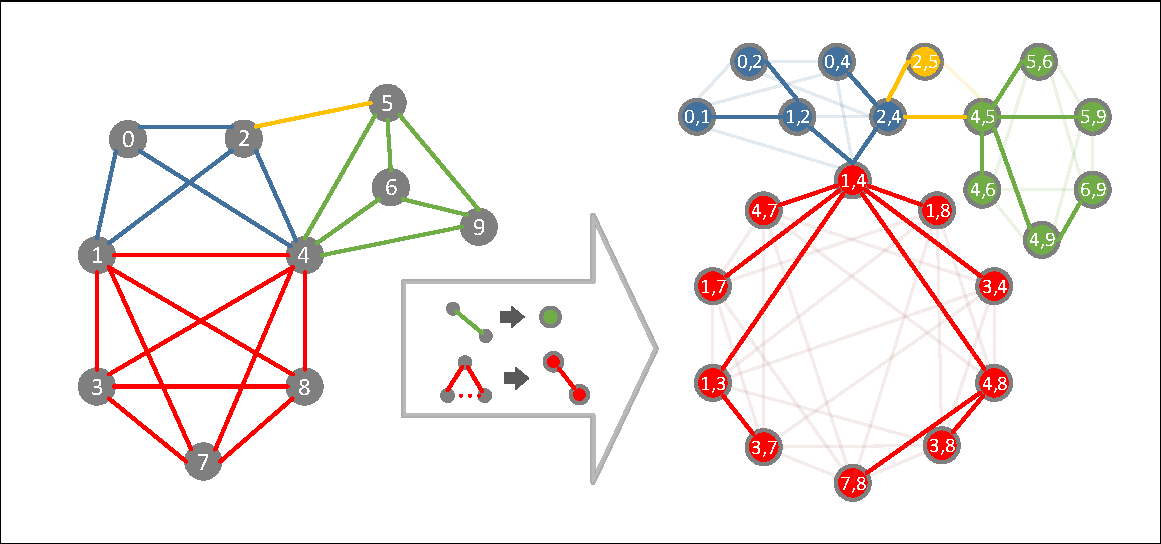
\includegraphics[width=0.8\linewidth, trim={0.1cm 0.1cm, 0.1cm, 0.1cm}, clip]{./figures/bottom_level.pdf}
    \caption{An example of the \inducedgraph{} and its maximum spanning tree of the example graph}
    \label{fig:\inducedgraph{}}
\end{figure}

We have the following theorem of vertex weights and edge weights in the \inducedgraph{}. 

\begin{Thm}
In \inducedgraph{} $G^m$, for a vertex $u$ and an adjacent edge $e$, we have $w_u \ge w_e$.
\label{thm:\inducedgraph{}_vertex_trussness}
\end{Thm}

\begin{proof}
According to \autoref{def:\inducedgraph{}}, $w_u$ is the trussness of the corresponding edge in $G_o$ while $w_e$ is the lowest trussness of edges in the corresponding triangle in $G_o$. 
%We have $\tau_{e} \ge \tau_{\triangle}$, therefore, $w_x \ge w_y$.
\end{proof}

We use $G^m$ to denote the maximum spanning forest of $G^t$ that has been stored as the bottom level index. To construct $G^m$, one way is generating the \inducedgraph{} $G^t$ first and then finding a maximum spanning tree of it. However, this approach is impractical because we need to sort edges in $G^t$ and the number of edges is three times the number of triangles of the original graph $G^o$, which can be an order of magnitude higher than the number of edges of most real-world graphs. We use two methods to avoid this. First, we find that for real-world graphs, the highest edge trussness is usually small compared to the size of the graph, \eg only a few thousand for the densest graph in our experiments. So we can use counting sort instead of comparison sort to reduce the time complexity. Second, as the weight of an edge of $G^t$ is the least trussness of edges in the corresponding triangle of $G^o$, we can sort edges of $G^o$ to generate edges of $G^t$ in sorted order with reduced space complexity. 
%This way, we can reduce the space complexity from $O(|{\triangle}^o|$ to $O({|E^o|})$. 
The details of the algorithm are shown in \autoref{alg:\inducedgraph{}_construction}. The algorithm takes $G^o$ and its edge trussness, which can be computed using the truss decomposition algorithm (\cite{wang2012truss}), as inputs.

\begin{algorithm}
	\KwData{$G^{o}(V^{o},E^{o})$, edge trussness $\{\tau_{e}, e \in E^{o}\}$}
	\KwResult{The \inducedgraph{} $G^{m}(V^{m}, E^{m})$}
	\BlankLine
	$sorted \gets$ sort edge trussness in decreasing order\;
	\For{$e \in E^{o}$} {
	   $V^{m} \gets V^{m} \bigcup \{e, \tau_{e}\}$\;
		 MAKE-SET($e$)\;
	}
	\For{$(u,v) \in sorted$}{
		suppose $u$ is the lower degree end of $(u,v)$\;
		\For{$w \in N_{u}$}{
			 \If{$(v,w) \in E^{o}$ \textbf{and} $\tau_{u,v} < \tau_{u,w}$ \textbf{and} $\tau_{u,v} < \tau_{v,w}$}{ 
				\Comment{Compare edge id if trussness of edges are equal to avoid duplication.}\;
				$\tau_{\triangle} = min(\tau_{(u,v)}, \tau_{(u,w)}, \tau_{(v,w)})$\;
				$E^{\triangle} \gets \{((u,v),(u,w)), \tau_{\triangle}\} \bigcup \{((u,v),(v,w)), \tau_{\triangle}\} \bigcup \{((u,w),(v,w)), \tau_{\triangle}\}$\;
				\For{$e^{\triangle} \in E^{\triangle}$}{
				  \If{FIND-SET($e^{\triangle}.v_1$) $\neq$ FIND-SET($e^{\triangle}.v_2$)}{
						$E^{m} \gets E^{m} \bigcup e^{\triangle}$\;
						UNION($e^{\triangle}.v_1$, $e^{\triangle}.v_2$)\;
					}
				}
			}
		}
	}
	\Return{$G^{m}(V^{m},E^{m})$}
	\caption{Bottom Level Index Construction}\label{alg:\inducedgraph{}_construction}
\end{algorithm}

The time and space complexity for computation of edge trussness of $G^o$ are $O(\sum_{(u,v) \in E^{o}}{min\{d_{u},d_{v}\}})$ and $O(|E^{o}|)$,  respectively. Sorting all the edges with counting sort costs $O(|E^{o}| + k_{max})$ time and $O(|E^{o}| + k_{max})$ space. The time and space complexity for listing all the triangles in $G^o$ is $O(\sum_{(u,v) \in E^{o}}{min\{d_{u},d_{v}\}})$ and $O(1)$, respectively. So the time and space complexity for generating the bottom level index when $k_{max} \ll |E^{o}|$ is $O(\sum_{(u,v) \in E^{o}} {min\{d_{u},d_{v}\}})$ and $O(|E^{o}|)$,  respectively. Since $G^m$ is a maximum spanning forest, the bottom level index takes $O(|V^{m}|) = O(|E^{o}|)$ space to store it.

\subsection{\TreeIndex{}}
\label{top-level}

\begin{figure}[ht]
    \centering
    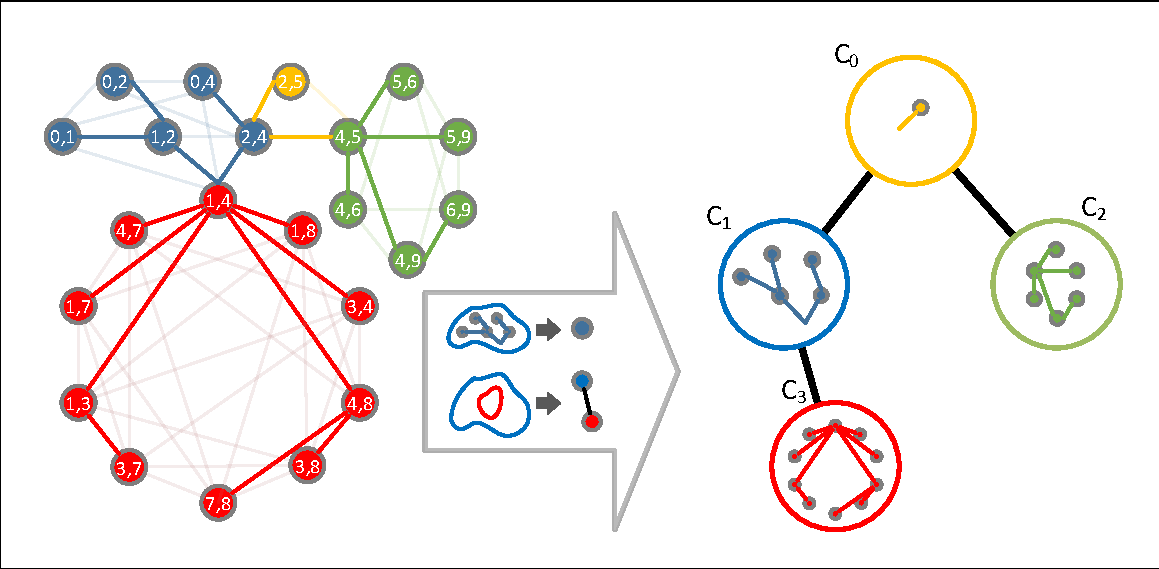
\includegraphics[width=0.8\linewidth, trim={0.1cm 0.1cm, 0.1cm, 0.1cm}, clip]{./figures/top_level.pdf}
    \caption{Overall structure of the \twolevelindex{}.}
    \label{fig:top-level}
\end{figure}

The top level index is extracted from k-truss communities and their relations in the original graph $G^o$ for fast locating relevant k-truss communities at query time. It is a super-graph having vertices represent unique k-truss communities and edges represent containment relations between k-truss communities. We call this index structure the \treeindex{} and denote it as $G^c$. Based on the hierarchical property of k-truss (\cite{cohen2008trusses}), \ie for $k \ge 2$, each $k$-truss is the subgraph of a ($k-1$)-truss, we have the formal definition of the \treeindex{} in \autoref{def:\treeindex{}}.

\begin{Def}[\Treeindex{}]
The \treeindex{} $G^c$ is a weighted undirected graph that each k-truss community in the original graph $G^o$ is represented by a vertex in $G^c$. $G^c$ has an edge $e^c$ connecting vertices $v^{c}_{1}, v^{c}_{2} \in G^{t}$ if and only if the following two conditions are met for their corresponding k-truss communities $C^{o}_{1}, C^{o}_{2} \in G^{o}$:
\begin{itemize}
	\item $C^{o}_{1}$ is a subgraph of $C^{o}_{2}$ or the other way around.
	\item Assume without loss of generality that $C^{o}_{1}$ is a subgraph of $C^{o}_{2}$, there is no $C^{o}_{3} \in G^{o}$ such that $C^{o}_{1}$ is a subgraph of $C^{o}_{3}$ and $C^{o}_{3}$ is a subgraph of $C^{o}_{2}$.
\end{itemize}
$G^c$ only has vertex weights, which are the trussness of the corresponding k-truss communities.
\label{def:\treeindex{}}
\end{Def}

A key property of the \treeindex{} is that it is a forest. 
%To prove this, we start with \autoref{thm:truss_hierarchy} 

%\begin{Thm}
%If k-truss community $C_{k1}$ is the subgraph of two other k-truss communities $C_{k2}$ and $C_{k3}$, respectively. We have $k2 \neq k3$.
%\label{thm:truss_hierarchy}
%\end{Thm}
%
%\begin{proof}
%According to \autoref{def:k-truss_community}, a k-truss community $C_{k1}$ is a subgraph of another k-truss community $C_{k2}$ when $C_{k1}$ and $C_{k2}$ are triangle connected and $k2 < k1$. Edges in $C_{k2}$ and $C_{k3}$ are triangle connected as they share the same k-truss community $C_{k1}$ as their subgraph. Suppose $k2 = k3$, $C_{k2} \bigcup C_{k3}$ meets the definition of k-truss community and becomes a larger k-truss community. This contradicts with $C_{k2}$ and $C_{k3}$ are maximal k-truss themselves.
%\end{proof}

\begin{Thm}
The \treeindex{} $G^c$ is a forest.
\label{thm:forest}
\end{Thm}

\begin{proof}
First, if there is a cycle $v^{c}_{1} ... v^{c}_{i} ... v^{c}_{n}$ in the \treeindex{} $G^c$ and their corresponding k-truss community in the original graph $G^o$ is $C^{o}_{1} ... C^{o}_{i} ... C^{o}_{n}$, respectively. According to \autoref{def:k-truss_community} and \autoref{def:\treeindex{}}, $C^{o}_{1} ... C^{o}_{i} ... C^{o}_{n}$ are triangle connected, and it is impossible for an arbitrary pair of community to have same trussness, as it contradicts with the maximal property of k-truss communities. Assume without loss of generality that vertex $v^{c}_{i}$ has the largest weight in this cycle, \ie its corresponding k-truss community $C^{o}_{i}$ has the smallest trussness. We denote the two adjacent vertices of it as $v^{c}_{j}$ and $v^{c}_{k}$. The corresponding k-truss communities are $C^{o}_{j}$ and $C^{o}_{k}$, respectively. By \autoref{def:\treeindex{}}, $C^{o}_{j}$ and $C^{o}_{k}$ are triangle connected. Assume without loss of generality that $C^{o}_{k}$ has smaller trussness than $C^{o}_{j}$, we have $C^{o}_{i}$ is a subgraph of $C^{o}_{j}$ and $C^{o}_{j}$ is a subgraph of $C^{o}_{k}$. So the edge between $v^{c}_{i}$ and $v^{c}_{k}$ contradict with the definition of the \treeindex{}.

Second, $G^c$ may have multiple connected components as not all k-truss communities in $G^o$ are triangle connected. 
\end{proof}

The \treeindex{} can be easily constructed with a single BFS traversal on the \inducedgraph{} $G^m$. For each connected component in $G^m$, the algorithm create a tree in the \treeindex{} $G^c$. The algorithm also creates a lookup table $H$ to map each vertex in $G^m$ to the super vertex in $G^c$ to which it belongs. \autoref{alg:\treeindex{}_construction} shows the detailed procedure. %Note that according to \autoref{thm:\inducedgraph{}_vertex_trussness}, an edge's weight is always smaller than it's endpoints' weights.

To construct each tree in $G^c$ with a connected component in $G^m$, the algorithm iteratively processes vertices during the BFS traversal and tracks the parent vertex $p^m$ of each vertex $u^m$.
To process a vertex $u^m$, the algorithm first compares weights, which are the trussness of corresponding edges in original graph $G^o$, of $u^m$ to its parent vertex $p^m$. The algorithm retrieves the super vertex $v^{c}_{p}$ using lookup table $H$, and find an ancestor super vertex with weight, which is trussness of the corresponding k-truss community in the original graph, smaller than the weight of $u^m$ if necessary. Depends on the relations of the weight of the found super vertex, the weight of the edge $(p^m, u^m)$ and the weight of vertex $u^m$, the algorithm decides whether to create a new super vertex in $G^c$ or assign $u^m$ to an existing super vertex.

\begin{algorithm}
	\KwData{$G^{m}(V^{m},E^{m})$}
	\KwResult{$G^{c}(V^{c},E^{c})$, $H$}
	\SetKwProg{Fn}{function}{}{end}
	\SetKw{Continue}{continue}
	\SetKw{Break}{break}
	\BlankLine
	%$Q \gets \emptyset$, $bfsparent \gets \emptyset$, $unvisited \gets V^{m}$\;
	%\While{$unvisited \neq \emptyset$}{
		%$seed \gets$ $unvisited.pop()$, $Q \gets Q \bigcup seed$; \Comment{Seed for new tree.}\
	\For{each connected component $CC \in G^m$} {
		$v^{m}_{seed} \gets CC.pop()$\;
		create\_super\_vertex($seed$, $null$)\;
		%\While{$Q \neq \emptyset$}{
			%$u^m = Q.pop()$\;
			%\For{$v^m \in N_{u^m} \bigcup unvisited$}{
				%$Q \gets Q \bigcup v^{m}$, $bfsparent[v^{m}] \gets u^{m}$, $unvisited.remove(v^{m})$\;
			%}
		\For{$u^m \in$ BFS starting at $seed$} {
			$p^m \gets$ parent of $u^m$ in BFS\;
			$e^m \gets (u^m, p^m)$\;
			$v^{c}_{p} \gets H[p^m]$\;
			%$p^m \gets bfsparent[u^m]$, $e^m \gets (u^m, p^m)$, $v^{s}_{p} \gets H[p^m]$\;
			\lWhile{$\tau_{v^{c}_{p}} > \tau_{e^m}$}{
				%\uIf{$\tau_{v^{s}_{p}} > \tau_{e^m}$}{
					${v^{c}_{p}}^{\prime} \gets v^{c}_{p}$, $v^{c}_{p} \gets v^{c}_{p}.parent$
					%\Continue
			}
			\eIf{$\tau_{v^{c}_{p}} < \tau_{e^m}$}{
				\eIf{$\tau_{e^m} = \tau_{u^m}$}{
					$v^{c}_{u} \gets$ create\_super\_vertex($u$, $v^{c}_{p}$)\;
					${v^{c}_{p}}^{\prime}.parent \gets v^{c}_{u}$\;
				} {
					$v^{c}_{e} \gets$ create\_super\_vertex($e$, $v^{c}_{p}$)\; 
					$v^{c}_{u} \gets$ create\_super\_vertex($u$, $v^{c}_{e}$)\;
					${v^{c}_{p}}^{\prime}.parent \gets v^{c}_{e}$\;
				}
			} {
				\eIf{$\tau_{e^m} = \tau_{u^m}$}{
					$H[u^m] \gets v^{c}_{p}$\;
				} {
					$v^{c}_{u} \gets$ create\_super\_vertex($u$, $v^{c}_{p}$)\;
				}
			}
		}
	}
	\Return{$G^{c}(V^{c},E^{c})$, $H$}
	\BlankLine
	\Fn{create\_super\_vertex ($u^m$, $v^{c}_{p}$)}{
		create $v^{c}_{u}$, $H[u^m] \gets v^{c}_{u}$\;
		$v^{c}_{u}.parent \gets v^{c}_{p}$\;
		$V^c \gets V^c \bigcup v^{c}_{u}$\;
		\Return{$C_u$}
	}
	\caption{Top Level Index Construction}
	\label{alg:\treeindex{}_construction}
\end{algorithm}

The reason we use the weight of the edge between a vertex and its parent vertex as the reference when adding a vertex of $G^m$ to $G^c$ can be explained by \autoref{thm:k_le_edge_weight}. 

\begin{Thm}
For a vertex $u^m$ and its neighbor vertex $v^m$ in the \inducedgraph{} $G^m$, if their representing edges in $G^o$ belong to the same k-truss community with the trussness of $k$, then $k \le \tau_{(u^m,v^m)}$. 
\label{thm:k_le_edge_weight}
\end{Thm}

\begin{proof}
Since $G^m$ is the maximum spanning forest, it has the cycle property, \ie for any cycle in the \inducedgraph{} $G^t$, if the weight of an edge in the cycle is smaller than the individual weights of all the other edges in the cycle, then this edge cannot belong to a maximum spanning forest. So there is no path in $G^t$ between $u^m$ and $v^m$ that has all edges with weight higher than $\tau_{(u^m,v^m)}$. Let $e^{o}_{u}$ and $e^{o}_{v}$ be their corresponding edges in original graph $G_o$, then $e^{o}_{u}$ is not triangle connected to $e^{o}_{v}$ in $G^o$ with edges that have trussness greater than $\tau_{(u^m,v^m)}$. Therefore, it is not possible for $e^{o}_{u}$ and $e^{o}_{v}$ to exist in the same k-truss community with trussness greater than $\tau_{(u^m,v^m)}$.
\end{proof}

For each vertex of $G^m$, searching the ancestor super vertex in $G^c$ of its parent vertex in $G^m$ takes $O(k_{max})$ time, where $k_{max}$ is the highest trussness of k-truss communities in $G^o$. Since the index construction process is a BFS on a maximum spanning tree with $O(|E^o|)$ vertices, the \treeindex{} construction algorithm takes $O(k_{max}|E^o|)$ time. As each vertex in $G^c$ represents a k-truss community in $G^o$, and $G^c$ is a forest. The algorithm takes $O(|E^o|)$ space and the index size is $O(|E^o|)$. %Although in practice, the size of $G^c$ is much smaller than $O(m)$.
%
%\begin{figure}[ht]
    %\centering
    %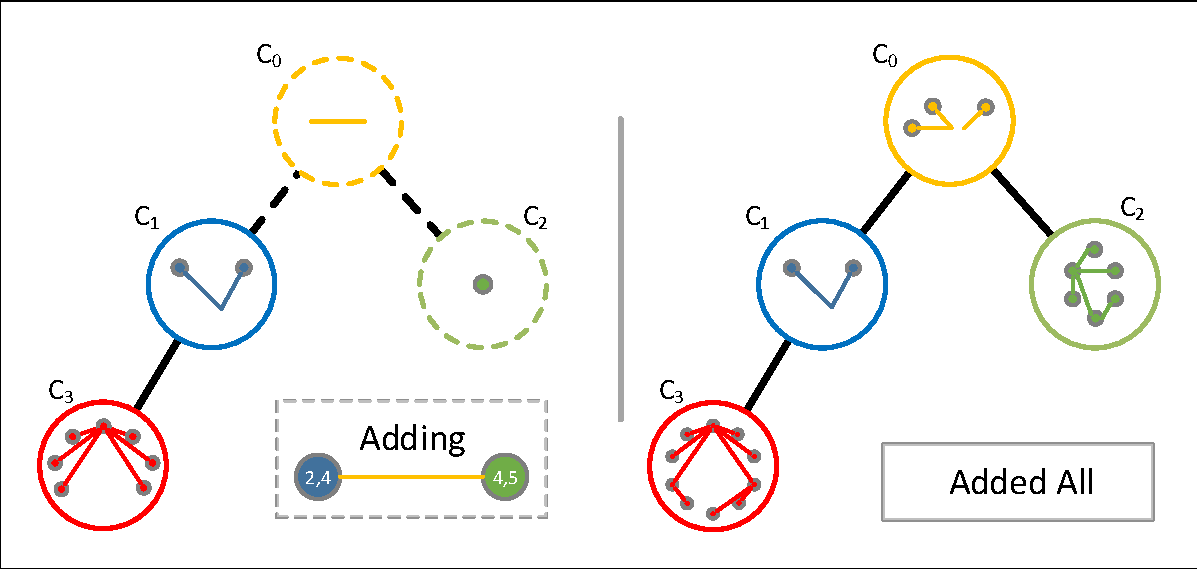
\includegraphics[width=\linewidth]{./figures/tree_index.pdf}
    %\caption{An example \treeindex{} of the \inducedgraph{} in \autoref{fig:\inducedgraph{}}}
    %\label{fig:\treeindex{}}
%\end{figure}
%
%An example is shown in \autoref{fig:\treeindex{}}

\subsection{\TwoLevelIndex Structure}
\label{structure}

\begin{figure}[ht]
    \centering
    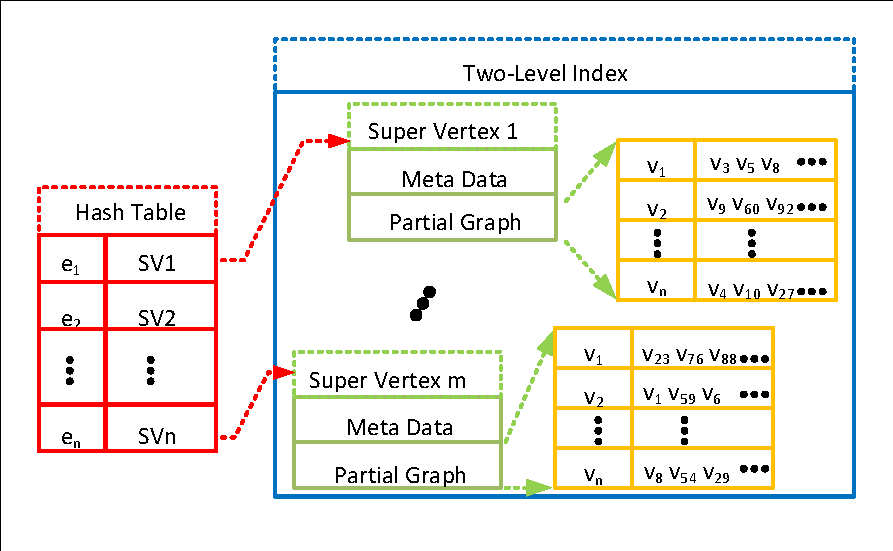
\includegraphics[width=0.8\linewidth, trim={0.1cm 0.1cm, 0.1cm, 0.1cm}, clip]{./figures/structure.pdf}
    \caption{Overall structure of the \twolevelindex{}.}
    \label{fig:structure}
\end{figure}

We combine the \inducedgraph{} and the \treeindex{} to form the \twolevelindex{} and arrange it in a structure that can provide information at different granularity. \autoref{fig:structure} shows an overview of the index structure. On the top level, we use an array to store the \treeindex{}. Each entry represents a single super vertex. Super edges are expressed by parent and children pointers. Within each entry, it also stores meta-data of the corresponding k-truss community, \eg the trussness, the community size, etc, for fast information retrieval. This meta-data can be gathered as a byproduct of index construction process. Finally, each entry contains a pointer of the data structure that stores part of the bottom level index. 

The bottom level index, which is the \inducedgraph{}, is stored as several separated adjacent lists. Each adjacent list contains edges of a single k-truss community that does not belong to any of its children k-truss communities. These adjacent lists can be easily generated as byproducts when constructing \treeindex{} using \autoref{alg:\treeindex{}_construction}. 
%Note that a vertex or edge in the \inducedgraph{} may belong to multiple k-truss communities. In these k-truss communities, k-truss communities with higher trussness is subgraphs of k-truss communities with lower trussness. To avoid redundancy, we only store the vertex and edge in the adjacent list of the k-truss community with the highest trussness. 

Finally, we have a hash table that maps each edge in the original graph to an entry in the top level of the \twolevelindex{}. One can also follow the similar fashion used in \cite{akbas2017truss}, which maps each vertex in the original graph to multiple entries in the top level index so that the original graph is not required during query time.

\section{Dynamic updates}
\label{dynamic}

This section describes update procedures of both \inducedgraph{} and \treeindex{} in dynamic graphs. We focus on edge insertion/deletion as vertex insert/deletion can be represented by inserting/deleting an isolated vertex and several following edge insertions/deletions.

The scope of affected edges when a new edge is inserted/deleted has been well studied in~\cite{huang2014querying}. When an edge $e_0$ has been added/removed from $G_o$, the affected edges, \ie with trussness changes, are either directly forming new triangles of weight $\ge \tau_{e_0}$ or are triangle connected to the new edge $e_0$ with all triangles of weight $\ge \tau_{e_0}$. With this rule, the authors of~\cite{huang2014querying} also developed an efficient algorithm to calculate edge trussness updates. 

We can then proceed to update the \inducedgraph{} $G_m$ once edge trussness in $G_o$ have been updated. For the insertion of an edge $e_0$, a new vertex $x_0$ is added to $G_{m}^{prime}$ with several new adjacent edges and updated weight of some vertices and edges. All we need to do is maintain the maximum spanning tree $G_m$ with these changes in $G_{m}^{prime}$. As maintaining Minimum spanning tree is a well studied area with highly efficient algorithms~\cite{cattaneo2002maintaining}, we omit the details here.

\note{are there problems if we dont update vertex and edges in order?}
Once we have updated $G_m$, we can proceed to update the \treeindex{} $G_t$. There are two types of changes for the update of $G_m$. One is vertex based that includes adding the new vertex $x_0$ and updating weights of other affected vertices. For a vertex $x$ that have updated weight, according to \autoref{thm:\inducedgraph{}_vertex_trussness}, the algorithm needs to create a new child vertex of current vertex $h[x]$ in $G_t$ based on the new weight. Note that this update is incomplete in the sense that we haven't taken into account the weight changes of the adjacent edges.  

\begin{algorithm}
	\KwData{An inserted/updated edge $(x, y) \in G_{m}$}
	\KwResult{None}
	\BlankLine
	$C_x \gets h[x]$, $C_y \gets h[y]$\;
	$k \gets w_{(x,y)}$\;
	\lWhile{$\tau_{C_x} > k$} {
		$C_x \gets C_{x}.parent$
	}
	\lWhile{$\tau_{C_y} > k$} {
		$C_y \gets C_{y}.parent$
	}
	$C \gets \emptyset$ \Comment{Assume $\tau_{\emptyset} = -1$.}\;
	\While{$C_x \neq \emptyset$ \textbf{or} $C_y \neq \emptyset$}{
		\uIf{$\tau_{C_x} > \tau_{C_y}$} {
			\lIf{$C \neq \emptyset$} {$C.parent \gets C_x$}
			$C \gets C_x$, $C_x \gets C_{x}.parent$\;
		}
		\uElseIf{$\tau_{C_x} < \tau_{C_y}$} {
			\lIf{$C \neq \emptyset$} {$C.parent \gets C_y$}
			$C \gets C_y$, $C_y \gets C_{y}.parent$\;
		}
		\Else{
			$C_c \gets$ combine ($C_x$, $C_y$)\;
			\lIf{$C \neq \emptyset$} {$C.parent \gets C_c$}
			$C \gets C_c$, $C_x \gets C_{x}.parent$, $C_y \gets C_{y}.parent$\;
		}
	}
	\caption{Zipper (Combine two branches)}\label{alg:zipper}
\end{algorithm}

Another type of change is that a new edge is added to $G_m$ or an edge has updated weight. This happens when a new triangle is formed in $G_o$ or the lowest trussness of edges in a triangle has changed. For a new edge $(x,y)$ in $G_m$, if $x$ and $y$ belongs to different connected components in $G_m$, then we need to combine the two branches of trees to which $h[x]$ and $h[y]$ belongs. We call this procedure zipper as shown in \autoref{alg:zipper}. In this way, K-Truss communities with trussness lower than the weight of the edge are combined together and the rest of high trussness communities become two separate children branch. 

\note{add a theorem here?} 
However, if a new edge is inserted in $G_m$ without join two disconnected parts, another edge with lower weight in $G_m$ must have been deleted to maintain the minimum spanning tree. In this case, if the two ends of the new edge $h[x]$ and $h[y]$ is different, we can still use zipper procedure to combine these two branches. The only difference is that we need to apply the zipper procedure from the least common ancestor of $h[x]$ and $h[y]$. Same goes for an edge with updated weight, as it can be viewed as deleting the edge with old weight and inserting a new edge with updated weight.

The update procedure for edge deletion in $G_o$ follows a similar process. It involves a vertex removal and vertex weight decreasing as well as several edge deletion and edge weight decreasing in $G_m$. Similarly, in $G_t$, we use a procedure to 'unzip' the branch of a deleted edge into two separate branches or a partially separated branch.

When using the zipper procedure to combine two branches (or divide one branch), we may have performance issues when updating the hashtable $h$. As one vertex change in $G_t$ may involve several entries to be updated in $h$. So how do we solve this problem....

\note{add time complexity analysis}

%Based on the update of the \inducedgraph{} $G_m$, we can update the \treeindex{} $G_t$. 
%\begin{itemize}
	%\item \textbf{Add a new edge in $G_o$} Add a new vertex in $G_m$. So only need to add a new vertex and create its own k-truss community in $G_t$ as it is not connected to any component in $G_m$ now.
	%\item \textbf{Form a new triangle in $G_o$} Add a new edge in $G_{m}^{prime}$. If such an edge is updated into the MST $G_m$, there might be another edge that has been deleted from $G_m$. However, in such a case, the connected components are still the same. But no matter the new edge connect two formerly disconnected components or not, the algorithm runs the same way. The algorithm can now combine two branch of the tree (or tree in case it connects two disconnected components) together. How? \note{define a procedure here} First find the LCA, and then check from the LCA, add each node with the lowest k from both side. If there are two nodes that has same k, combine them and add the combined node to the tree.
	%\item \textbf{a triangle has trussness update in $G_o$} An edge has weight update in $G_{m}^{prime}$. If such an edge does not belongs to $G_m$ previously, and now becomes an edge in $G_m$, same as adding a new edge. Otherwise, As from \autoref{thm:\inducedgraph{}_vertex_trussness}
	%
%\end{itemize}

\section{Evaluations}
\label{evaluation}

In this section, we evaluate our proposed index structure for various types of k-truss community related queries on real-world networks. We first compare the \twolevelindex{} with state-of-the-art solutions, the TCP index (\cite{huang2014querying}) and the Equitruss index (\cite{akbas2017truss}) for index construction (Section~\ref{eval_const}) and single vertex k-truss community search (Section~\ref{eval_singlev_k_compare}). Then we show the effectiveness of our index for all three types of \toplevelprob{} k-truss community queries and their corresponding k-truss community search with single and multiple query vertices (Section~\ref{eval_top_bottom_compare} \& Section~\ref{eval_k_type_compare}). Finally, we analyze results of \bottomlevelprob{} k-truss community queries (Section~\ref{eval_bottom_analysis}). All experiments are implemented in C++ and are run on a Cloudlab\footnote{www.cloudlab.us} c8220 server with 2.2GHz CPUs and 256GB memory. 
%\subsection{Datasets}
\vskip 0.1in \noindent \textbf{Datasets} 

\begin{table}
\caption{Datasets}
\label{table:datasets} 
\begin{threeparttable}
	\centering
		\begin{tabularx}{\linewidth}{c|*{5}{Y}} 
		\toprule
			Dataset & Type & $|V_{wcc}|$ & $|E_{wcc}|$ & $|{\triangle}_{wcc}|$ & $k_{max}$ \\
			\midrule
			Wiki & Comm. & 2.4M & 4.7M & 9.2M & 53 \\ 
			Baidu & Web & 2.1M & 17.0M & 25.2M & 31 \\
			Skitter & Internet & 1.7M & 11.1M & 28.8M & 68 \\ 
			Sinaweibo & Social & 58.7M & 261.3M & 213.0M & 80 \\ 
			Livejournal & Social & 4.8M & 42.8M & 285.7M & 362 \\ 
			Orkut & Social & 3.1M & 117.2M & 627.6M & 78 \\
			Bio & biological & 42.9K & 14.5M & 3.6B & 799 \\
			Hollywood & Collab. & 1.1M & 56.3M & 4.9B & 2209 \\
			%Webuk & Web & 39.3M & 796.4M & & \\ 
			%Friendster & Social & 65M & 1.8B & & \\
			\bottomrule
			\end{tabularx}
			\begin{tablenotes}
				\item Datasets with the number of vertices, edges, triangles and the maximum trussness ($k_{max}$) in the largest weakly connected components without self edges. Sorted by the number of triangles.
			\end{tablenotes}
		\end{threeparttable}
\end{table}

We use 8 real-world graphs of different types as shown in the Table~\ref{table:datasets}. To simplify our experiments, we treat them as undirected, un-weighted graphs and only use the largest weakly connected component of each graph. We also removed all the self edges in each graph. 
%We sort the graph according to their number of triangles as ktruss community highly relies on triangles in the graph. 
All datasets are publicly available from Stanford Network Analysis Project\footnote{snap.stanford.edu} and Network Repository\footnote{networkrepository.com}.

\subsection{Index construction}
\label{eval_const}

\begin{table}
		\caption{Comparison of Index Construction}
		\label{table:index_construction}
		\centering
		%\begin{tabular}{|c|c|ccc|ccc|} \hline 
		%& Graph & \multicolumn{2}{|c|}{Index Size} & \multicolumn{2}{|c}{Index Time} \\
			%\cline{3-6}
			\begin{tabularx}{\linewidth}{c c *{6}{Y}}
			\toprule
			Graph & Decomp.
						& \multicolumn{3}{c}{Index Time (Sec.)} 
						& \multicolumn{3}{c}{Index Size (MB)} \\
			\cmidrule(lr){3-5} \cmidrule(l){6-8}
			 Name & Time (Sec.) & TCP & Equi & Our & TCP & Equi & Our \\ 
			\midrule
			Wiki & 239 & 139 & 63 & 83 & 58 & 25 & 32 \\ 
			Baidu & 742 & 494 & 269 & 350 & 306 & 179 & 237 \\
			Skitter & 366 & 167 & 151 & 139 & 139 & 240 & 193 \\ 
			Sinaweibo & 10728 & 11048 & 5724 & 6871 & 2744 & 1390 & 1810 \\
			Livejournal & 2201 & 1313 & 795 & 1020 & 1129 & 585 & 844 \\ 
			Orkut & 9028 & 7659 & 3609 & 5059 & 3302 & 1722 & 2479 \\
			Bio & 11239 & 13964 & 6223 & 8874 & 393 & 177 & 289 \\
			Hollywood & 14002 & 16620 & 4154 & 10182 & 1929 & 813 & 1276 \\ 
			
			%Wiki & 57.5 & 138.6 & 62.8 & 83.3 & 58.4 & 24.9 & 32.4 \\ 
			%Baidu & 224.5 & 493.9 & 268.5 & 350.3 & 305.8 & 179.0 & 237.3 \\
			%Skitter & 149.1 & 166.9 & 151.1 & 138.5 & 138.6 & 239.7 & 192.7 \\ 
			%Sinaweibo & 4049.9 & 11047.6 & 5724.3 & 6870.7 & 2743.8 & 1390.0 & 1810.4 \\
			%Livejournal & 627.6 & 1312.9 & 794.9 & 1020.0 & 1128.8 & 585.3 & 844.1 \\ 
			%Orkut & 1769.8 & 7659.4 & 3609.1 & 5058.7 & 3301.6 & 1721.8 & 2479.0 \\
			%Bio & 165.7 & 13963.9 & 6222.7 & 8873.6 & 393.1 & 176.6 & 289.4 \\
			%Hollywood & 791.7 & 16619.7 & 4154.4 & 10181.7 & 1928.7 & 812.5 & 1276.3 \\ 
			%Webuk & 13999 &   &  &  & \\ 
			%Friendster & 32364 &   &  &  & \\
			\bottomrule
		\end{tabularx}
\end{table}

We show in this section the index size and index construction time of the \twolevelindex{} compared to the TCP index and the Equitruss index in 
Table \ref{table:index_construction}. 
%Both indices are generated in memory and we show the size of the data structures that hold the index. 
We exclude the truss decomposition time for all three methods so that the index construction time only shows how long it takes to generate a certain index with edge trussness provided. 
We can see in Table \ref{table:index_construction} that the \twolevelindex{} has comparable construction time to the Equitruss index and both are faster than the TCP index. The index size of the \twolevelindex{} is smaller than the TCP index as there are no repeating edges stored in the index. However, the Equitruss has the smallest index size since it only stores edge list of the original graph while the \twolevelindex{} also stores the edges alongside vertices, which preserves the triangle connectivity inside k-truss communities. Note that if only \toplevelprob{} k-truss community queries are processed, the algorithm only needs to retrieve the top level index which has a much smaller size. %Note that the provided size is the minimum size to store the required index, the actual size may vary due to different implementations. 

\subsection{Query performance}
\label{eval_query_time}

In this section, we evaluate the query time of various query types to show the effectiveness of the \twolevelindex{}. As k-truss community query time heavily relies on the degree of query vertices, we use a similar procedure as used by \cite{huang2014querying} to partition vertices to be used in the experiments. Because only vertices with a degree of $k + 1$ can appear in a k-truss community with trussness of $k$. If we partition vertices uniformly by their degree and the graph has highly screwed degree distribution, then vertices in most of the partitions would have a too low degree to appear in a k-truss community. To show the performance of different algorithms on mining community structures in this kind of graphs, we fix the trussness of k-truss community search queries at $10$ and discard vertices with degree less than $20$. Then we uniformly partition the rest of vertices according to their degrees into 10 categories and at each category, we randomly select 100 sets of query vertices.

%\vskip 0.1in \noindent \textbf{Single vertex k-truss community search.}
\subsubsection{Single vertex k-truss community search.}
\label{eval_singlev_k_compare}

\begin{figure*}[t]
    \centering
    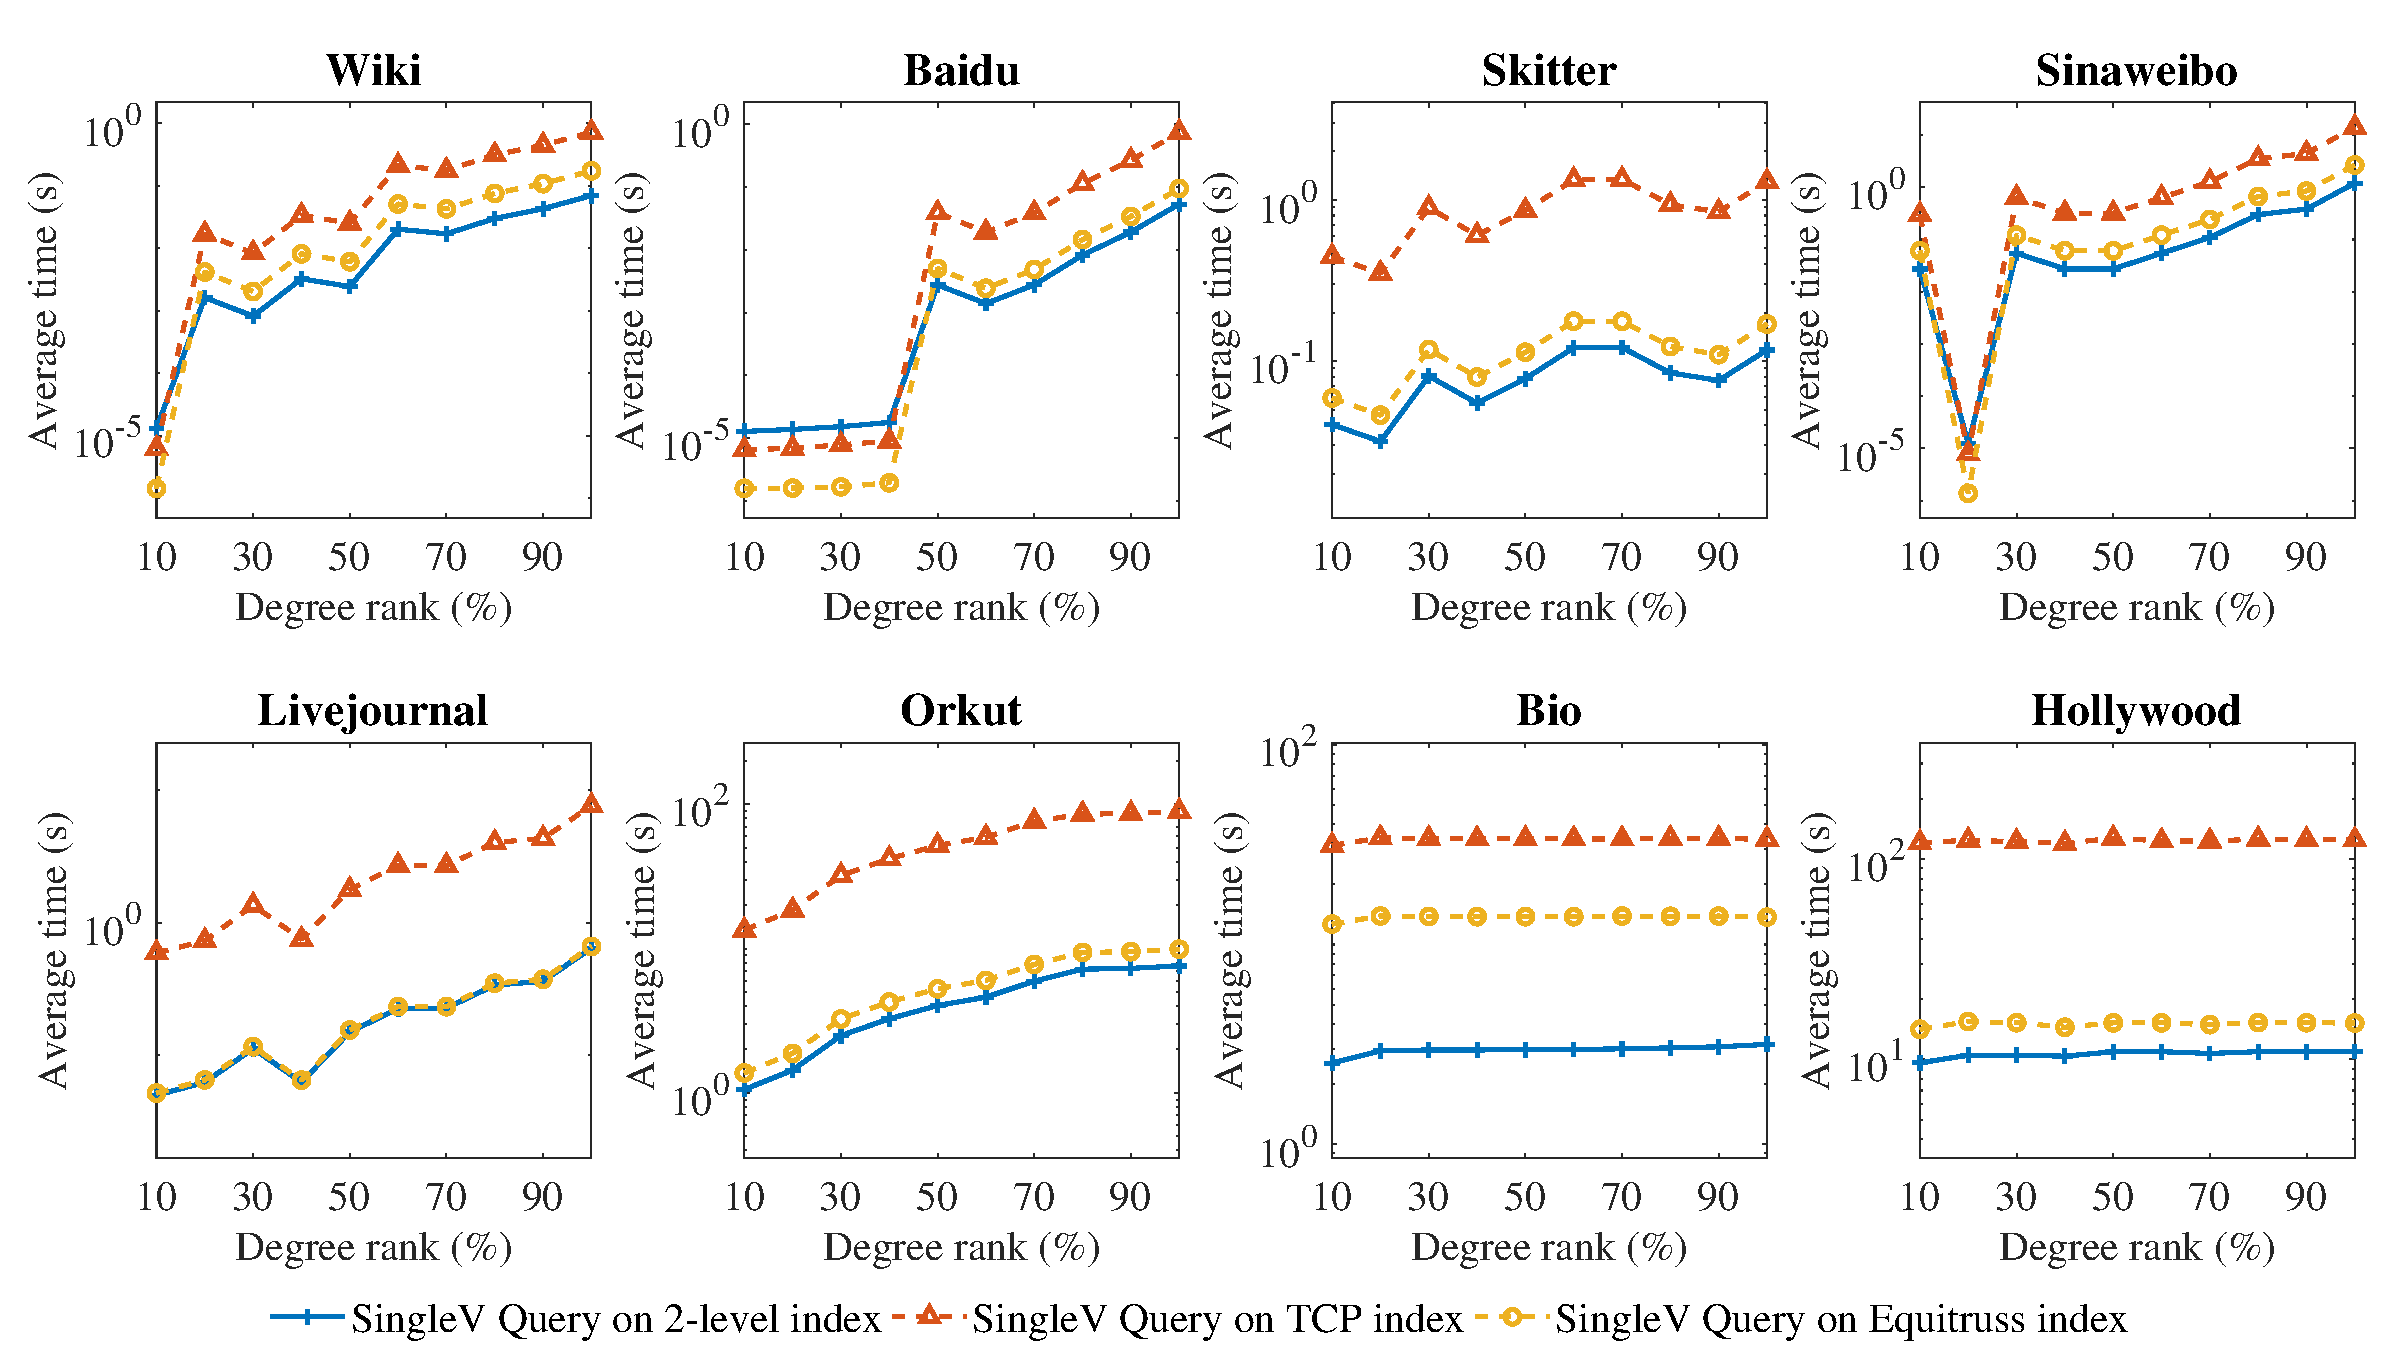
\includegraphics[width=0.8\textwidth]{./figures/singlev_k_compare.pdf}
    \caption{Comparison of single vertex k-truss community search of the \twolevelindex{}, the TCP index and the Equitruss index.}
    \label{fig:singlev_k_compare}
\end{figure*}

We first evaluate the single vertex k-truss community search performance and compare the query time with the TCP index and the Equitruss index. The results are shown in \autoref{fig:singlev_k_compare}. The \twolevelindex{} achieves best average query time for all graphs. It has an order of magnitude speedup compared to the TCP index for all graphs and $5\%$ to $400\%$ speedup compared to the Equitruss index for all graphs. However, the speed up is linear as all three indices have the same time complexity to handle single vertex k-truss community search queries. Note that very low average query time (around $10^{-5}$ second) means there is no vertex belonging to any k-truss community in that degree rank.

\begin{figure}[h]
\centering
\subfigure[Number of vertices in super-graphs.\label{fig:graphsize_vertices}]{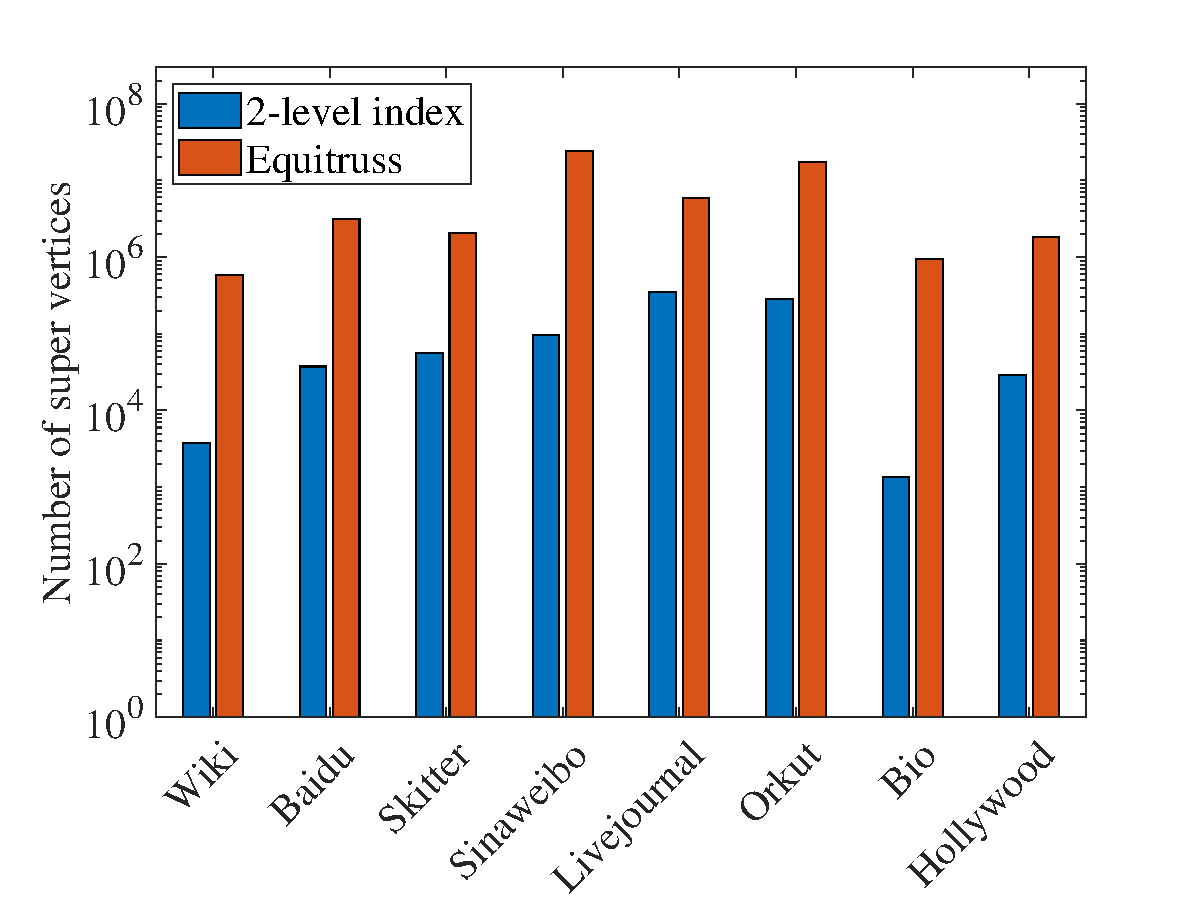
\includegraphics[width=0.45\linewidth]{./figures/super_node_compare.pdf}}
\subfigure[Number of edges in super-graphs.\label{fig:graphsize_edges}]{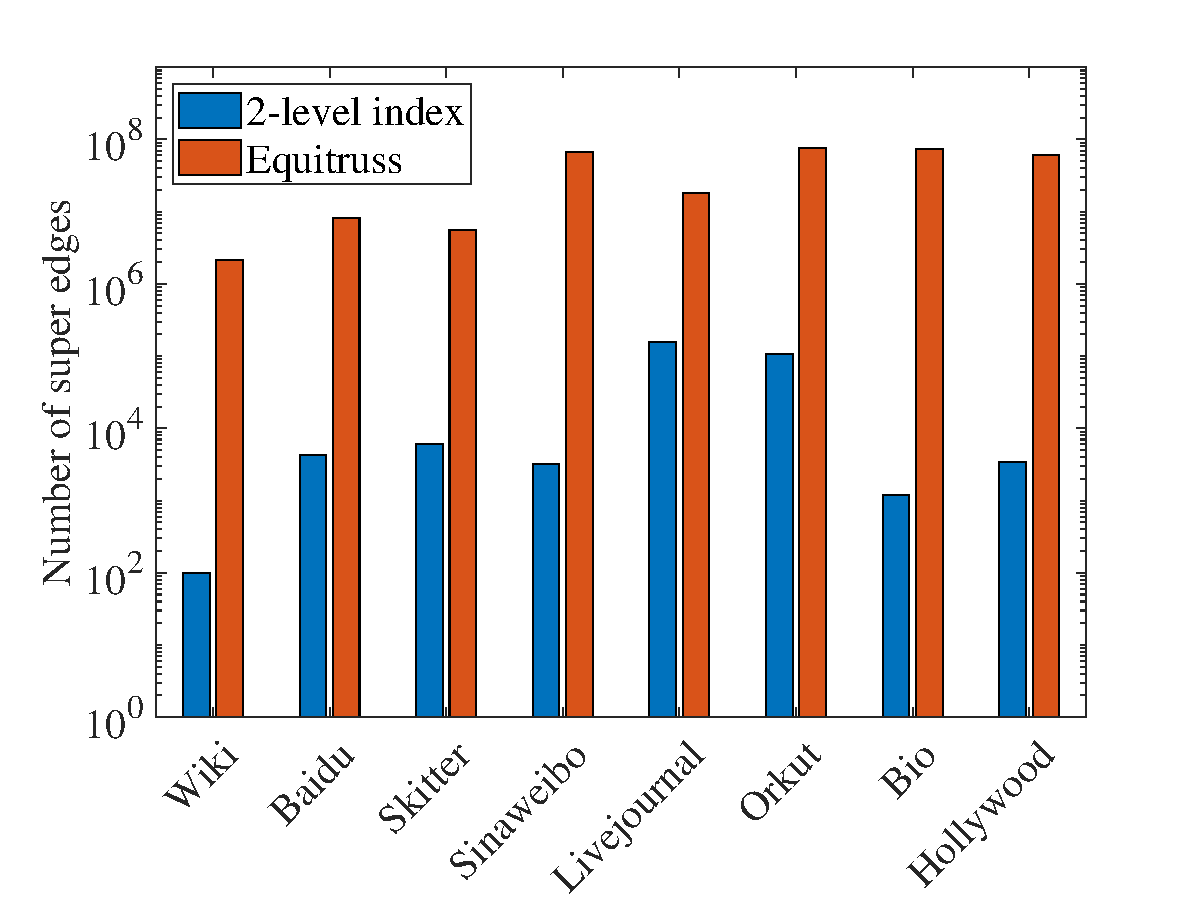
\includegraphics[width=0.45\linewidth]{./figures/super_edge_compare.pdf}}
\caption{Super-graph size comparison of the \twolevelindex{} and the Equitruss index.}
\label{fig:graphsize}
\end{figure}

\vskip 0.1in \noindent \textbf{Reason of performance difference.} The main reason that the \twolevelindex{} is faster than the TCP index is the avoidance of the expensive BFS search during query time. The reason for performance differences of the \twolevelindex{} and the Equitruss index on various graphs is less obvious given that they both search for target communities on a super-graph of the original graph and then collect edges belonging to the target community. The difference lies in the fact that vertices and edges in the super-graph of the two indices represent different subgraphs and their relations of the original graph. Each vertex in the \twolevelindex{} represents a single k-truss community while vertices in the Equitruss index only represents a fraction of a k-truss community. So one vertice in \twolevelindex{} may be split into several vertices in the Equitruss index. 

We show the super-graph sizes of the \twolevelindex{} and the Equitruss index in \autoref{fig:graphsize}. We can see that the size of the super-graph of the Equitruss index is an order of magnitude larger than the super-graph of the \twolevelindex{}. The Equitruss index is slow while finding target communities due to the larger super-graph size. However, edge lists of a k-truss community can be more effectively retrieved as it is already stored in each super vertex. For the \twolevelindex{}, target communities are easier to identify, however, one need to iterate through the adjacent lists stored in super vertices to retrieve edges in the community. % and then convert vertices of the \inducedgraph{} back to their corresponding edges in the original graph. %Now it's not hard to understand the performance different on different real-world graphs, 

\subsubsection{The \toplevelprob{} query $vs.$ the \bottomlevelprob{} query (community search).}
\label{eval_top_bottom_compare}

\begin{figure*}[t]
    \centering
    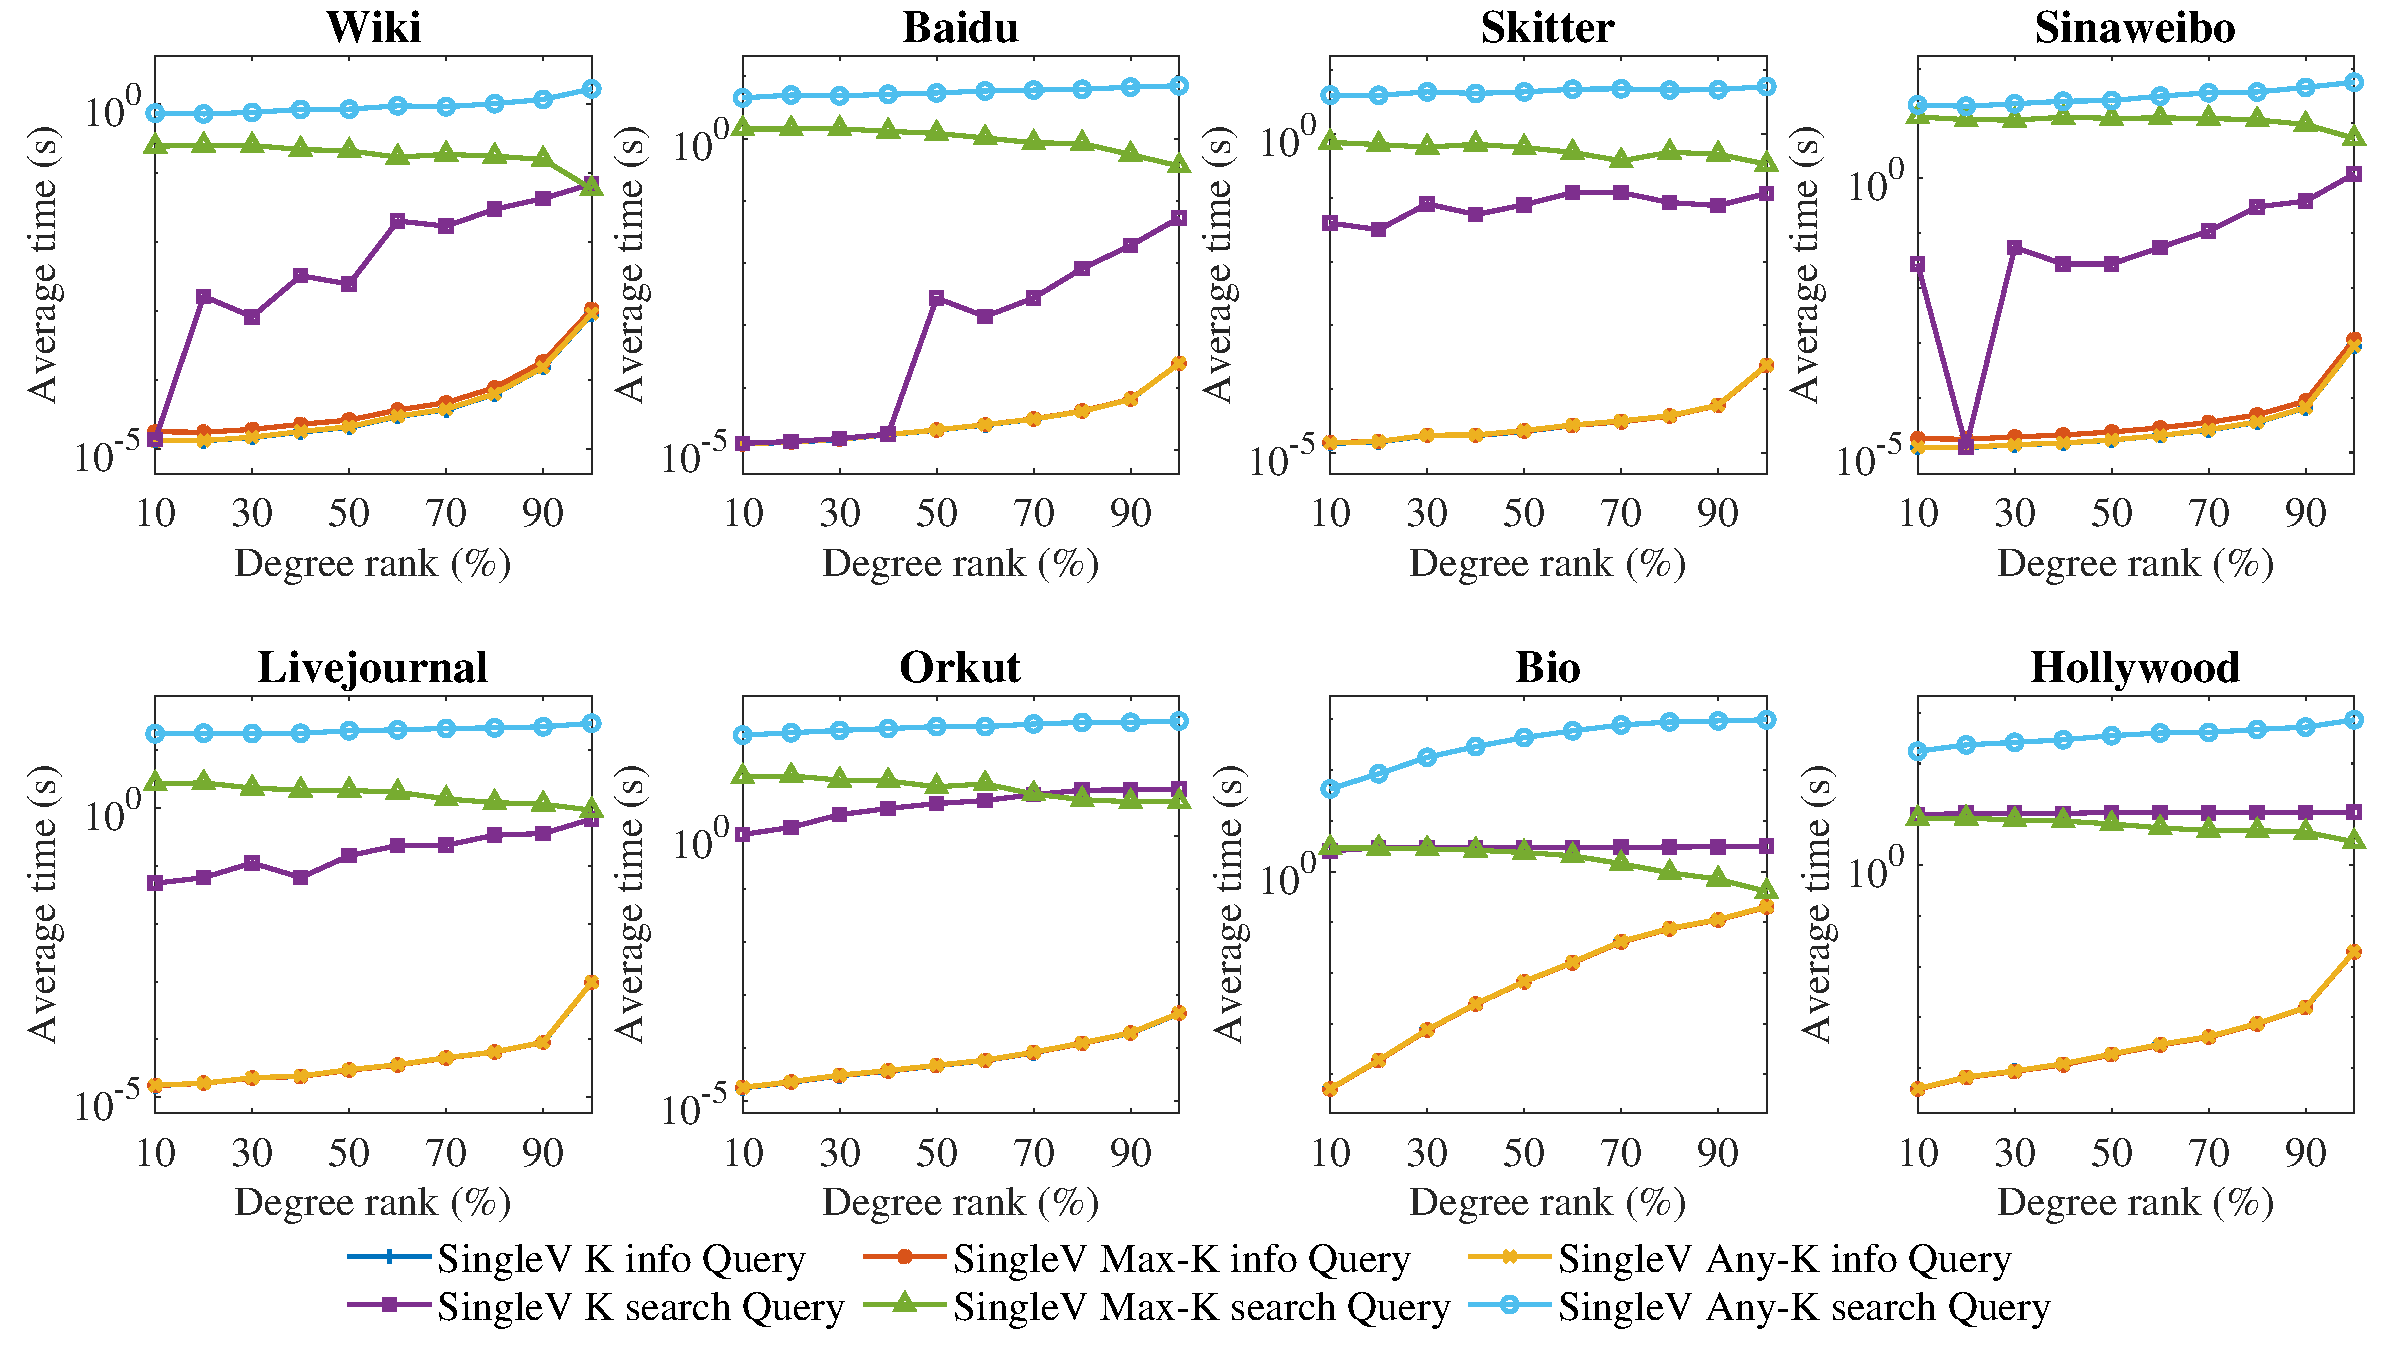
\includegraphics[width=0.8\linewidth]{./figures/singlev_info_query.pdf}
    \caption{Three types (k-truss, max-k-truss, any-k-truss) of single-vertex \toplevelprob{} k-truss community query $vs.$ community search.}
    \label{fig:singlev_info_query}
\end{figure*}

%\begin{figure}[ht]
    %\centering
    %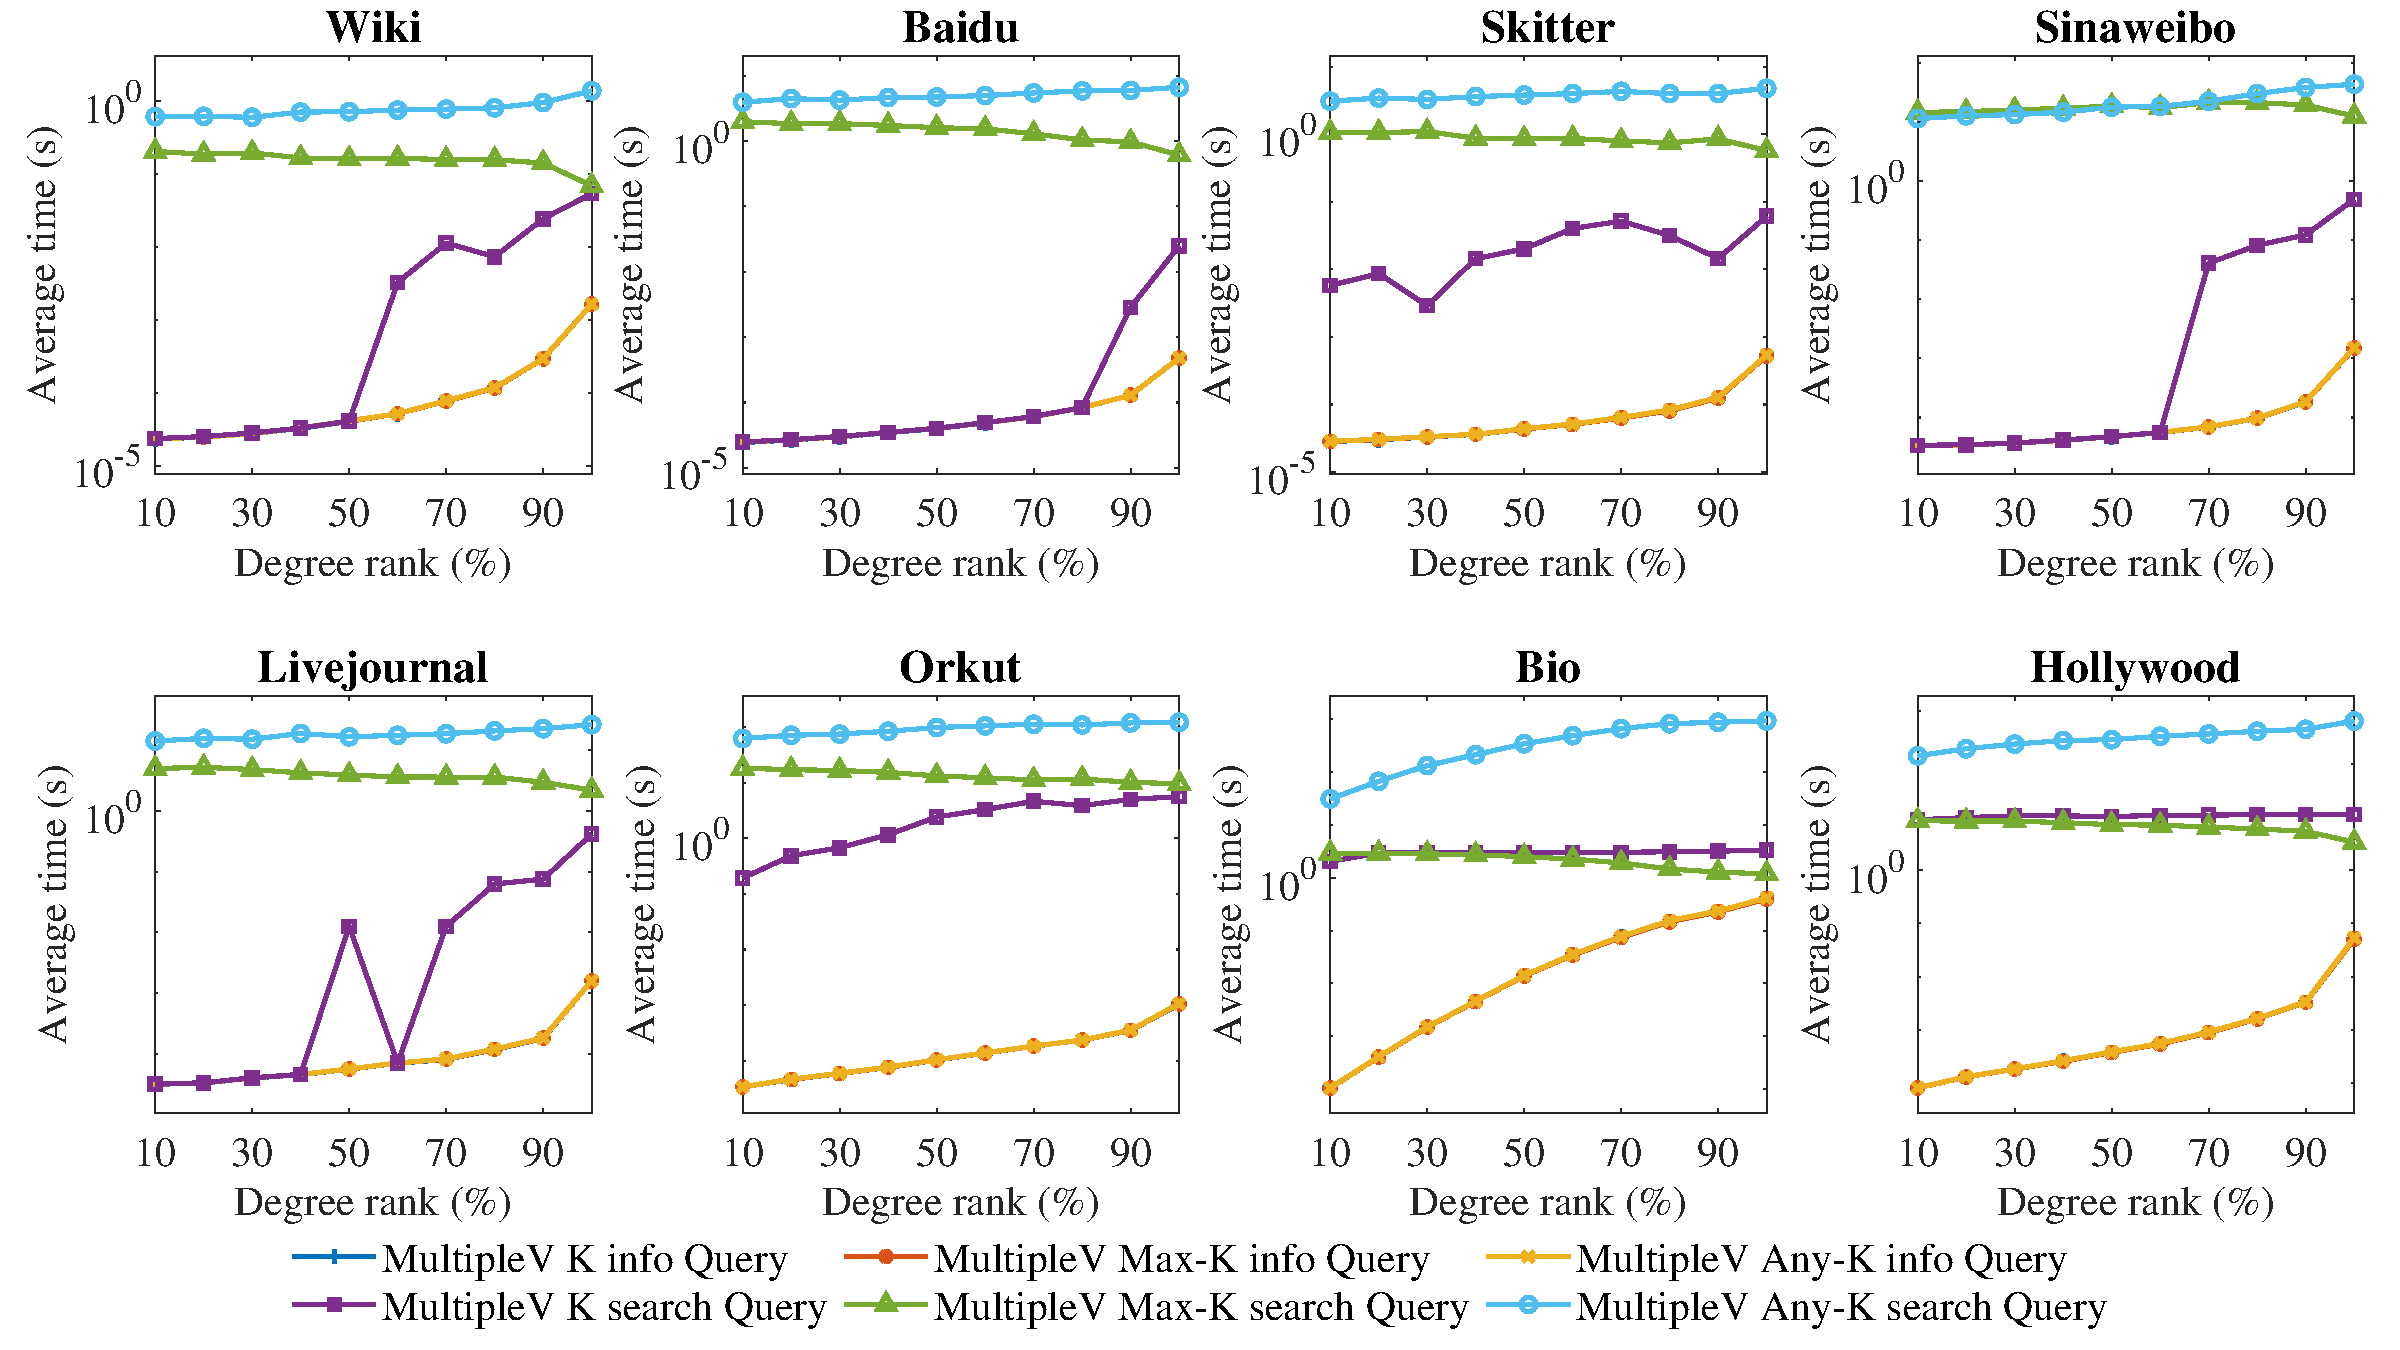
\includegraphics[width=\linewidth]{./figures/multiplev_2_info_query.pdf}
    %\caption{Single vertex query for exact truss community search.}
    %\label{fig:multiplev_2_info_query}
%\end{figure}

\begin{figure*}[t]
    \centering
    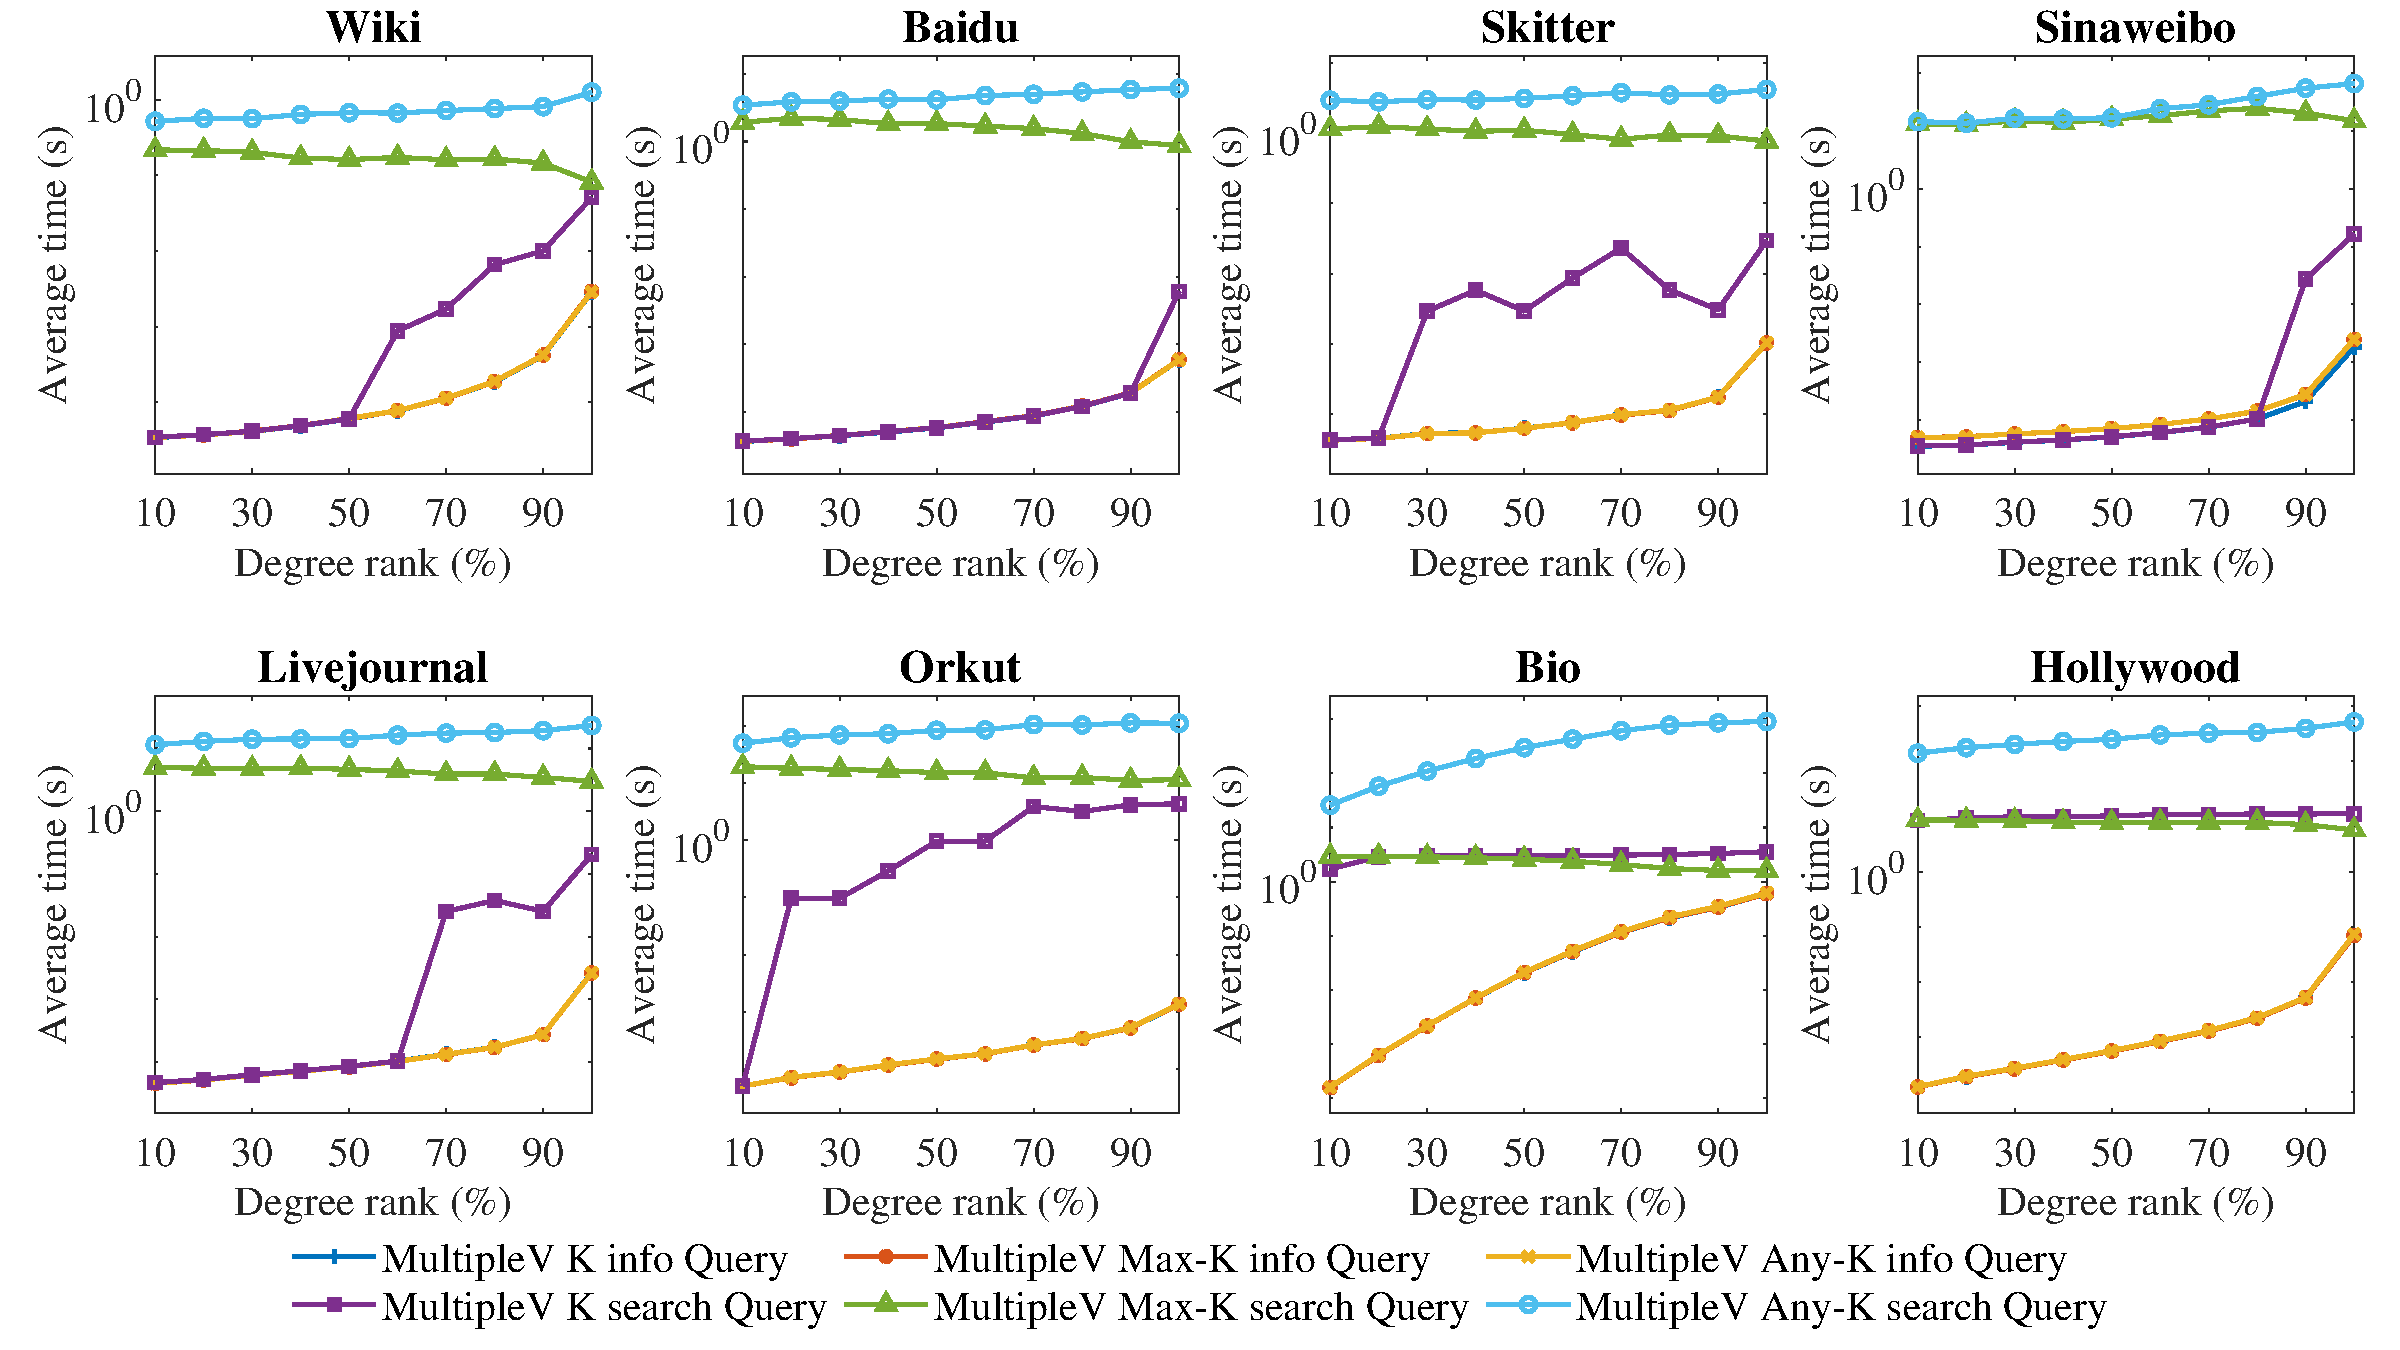
\includegraphics[width=0.8\linewidth]{./figures/multiplev_3_info_query.pdf}
    \caption{Three types (k-truss, max-k-truss, any-k-truss) multiple-vertex ($3$) \toplevelprob{} k-truss community query $vs.$ community search.}
    \label{fig:multiplev_3_info_query}
\end{figure*}

We perform all three basic types, \ie k-truss, max-k-truss and any-k-truss, of \toplevelprob{} k-truss community queries and perform community search queries on the targeting communities found by \toplevelprob{} queries. We show both single-query-vertex cases and multiple-query-vertex ($3$ vertices) cases in \autoref{fig:singlev_info_query} and \autoref{fig:multiplev_3_info_query}, respectively. 

%\vskip 0.1in \noindent \textbf{\toplevelprob{} query $vs.$ \bottomlevelprob{} query (community search).} 
We can see in both figures that our index is very effective for both \toplevelprob{} queries and community search queries. The average time for \toplevelprob{} queries spans from $1.22 x 10^{-5}$ second to $0.62$ second. The average time for community search queries is typically much higher than \toplevelprob{} queries since it needs to access edge level information, ranging from $2.20 x 10^{-5}$ to $979.81$ seconds depending on the size of target communities. The multi-hundred average run time comes from searching all truss communities that contain a query vertex (any-k-truss query) with a very high degree in the densest graph (bio). The fast query time of \toplevelprob{} queries makes it an excellent candidate for applications that require community-relation information such as whether a set of vertices belong to the same k-truss communities without digging into the details of any k-truss community. 

\subsubsection{K-truss query $vs.$ max-k-truss query $vs.$ any-k-truss query.}
\label{eval_k_type_compare}

%\vskip 0.1in \noindent \textbf{K-truss query $vs.$ max-k-truss query $vs.$ any-k-truss query.} 
We can also see in \autoref{fig:singlev_info_query} and \autoref{fig:multiplev_3_info_query} any-k-truss community search queries always have the highest average run time because it searches all the possible truss communities to which the query vertex/vertices belong. We can also see that k-truss community search queries usually have much smaller average run time than max-k-truss community search queries. 
%Is it because the index are more effective for k-truss community search query? Not really. 
%When checking the search result data, we find 
It is because that many k-truss queries fail to find a truss community as the query vertex/vertices do not belong to any truss community with the specified $k$, which is $10$ in our experiments. However, this problem is less severe for max-k-truss queries. Max-k-truss queries can always find a target community as long as the query vertex/vertices belong to any truss community. In most cases, max-k-truss queries can provide more useful information for applications that do not have much knowledge of the community structure in the underlying graph.

Another interesting trend is that as the degree of query vertex increases, the average run time for k-truss and any-k-truss community search queries increases, the average run time for max-k-truss queries decreases. The trend is caused by different reasons for three types of query. For k-truss queries, the average query time increases as the query vertex degree increases because that it is more likely to find a target k-truss community with the specified $k$, which is $10$ in our experiments. For max-k-truss queries, the average query time decreases as the query vertex degree increases because that target truss communities have higher trussness and smaller size. For any-k-truss queries, because the k-truss communities have hierarchical structures, more truss communities will be discovered by a query so that the average query time increases when the query vertex degree increases.

\subsection{\BottomLevelProb{} Query Analysis}
\label{eval_bottom_analysis}

%\begin{figure}[h]
%\centering
%\subfigure[Boundary search.\label{fig:boundary}]{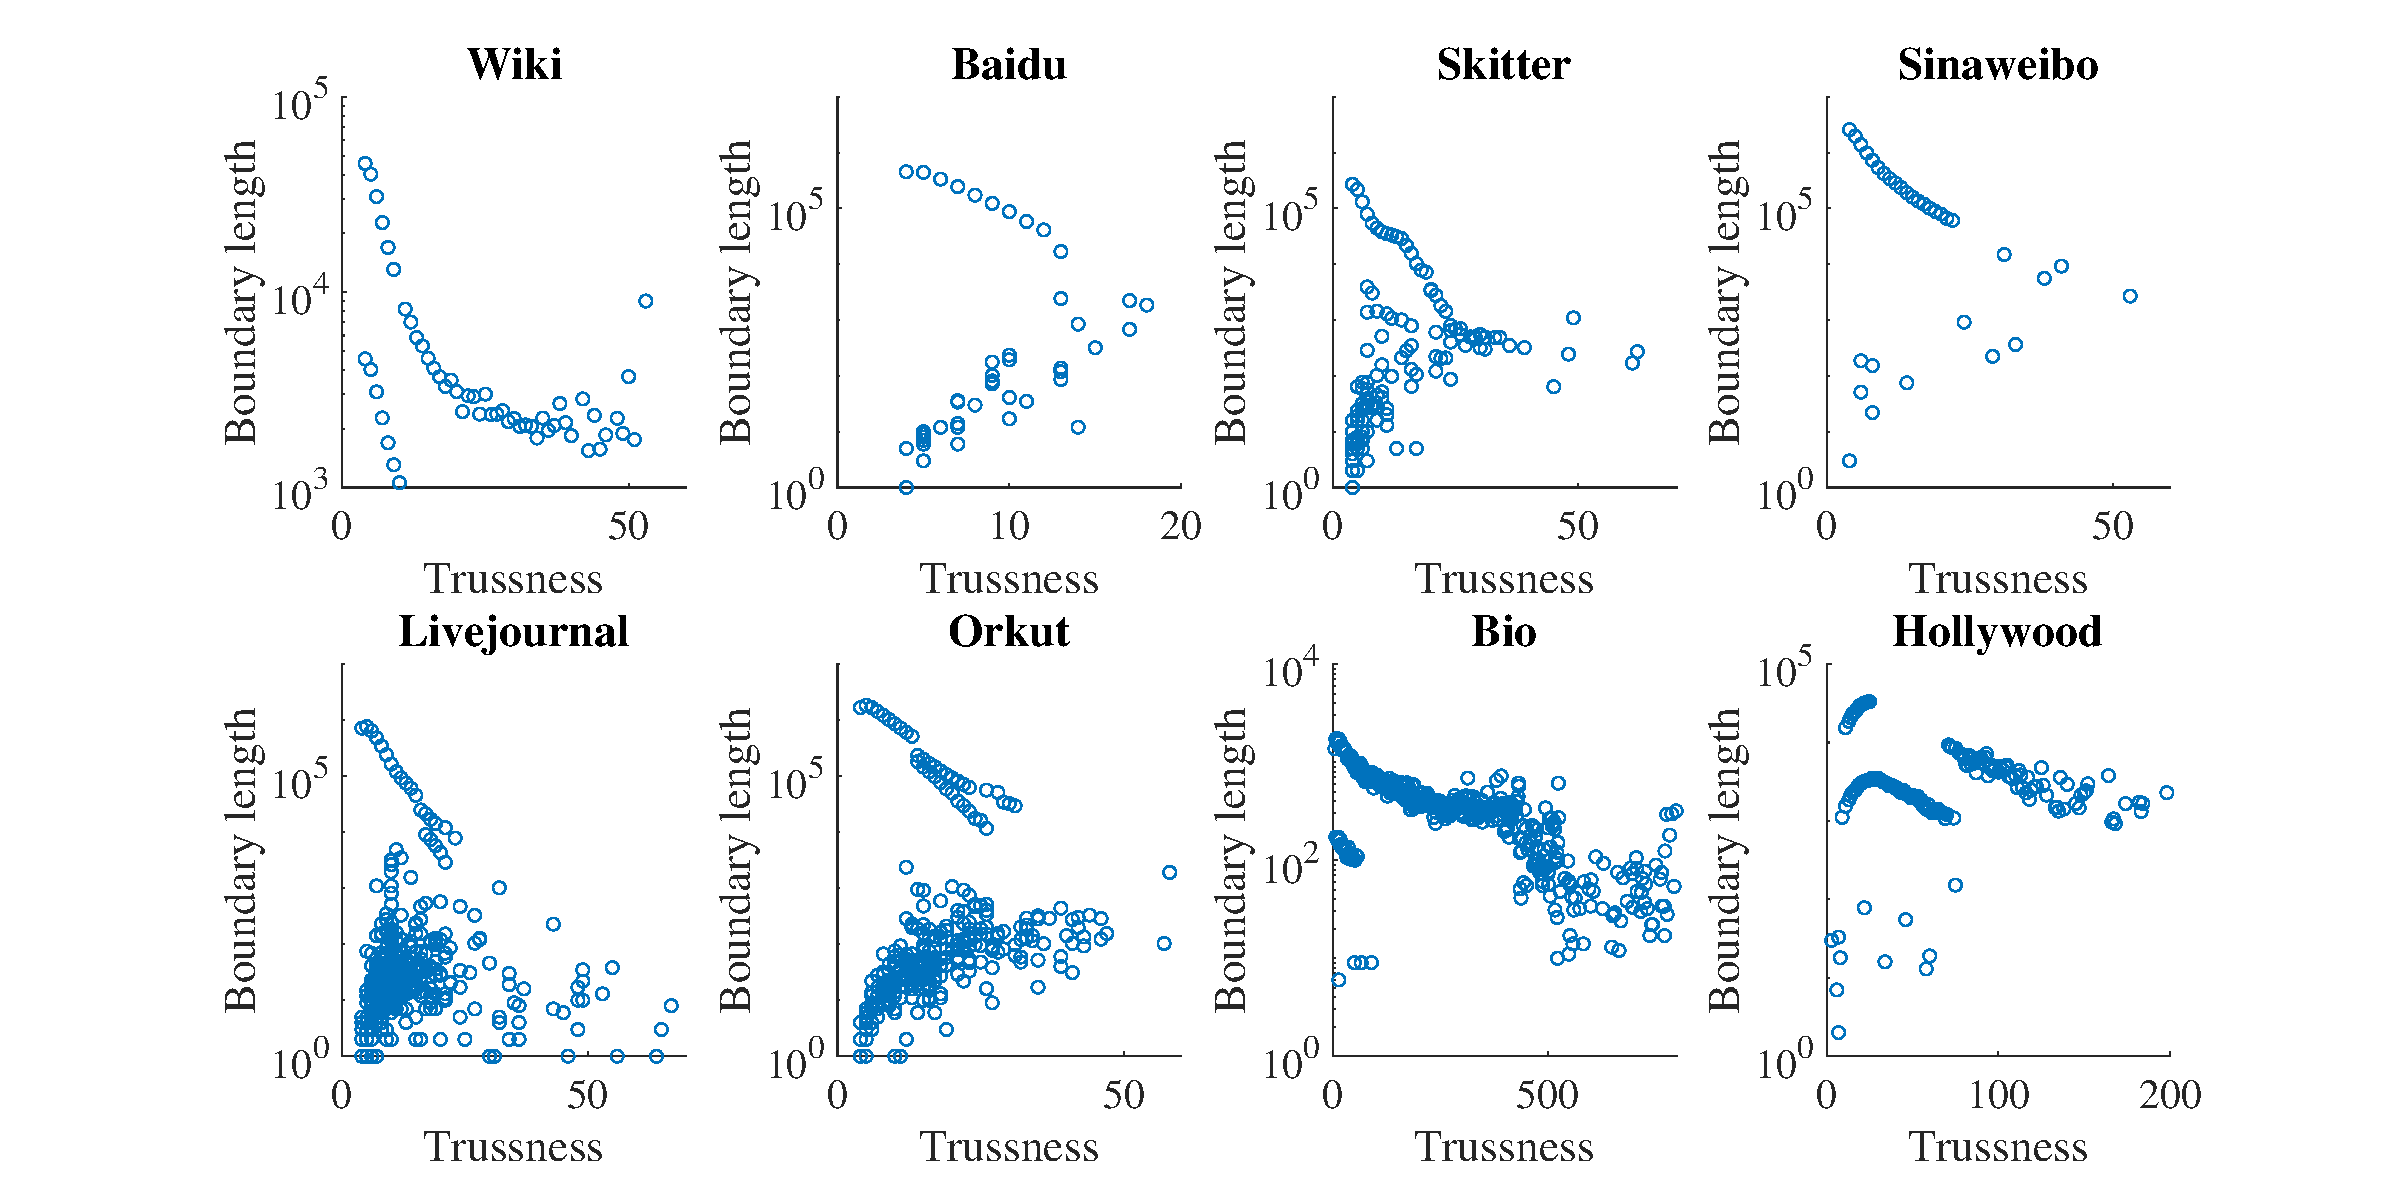
\includegraphics[width=0.78\linewidth]{./figures/boundary_size.pdf}}
%\subfigure[Maximim triangle connected path.\label{fig:path}]{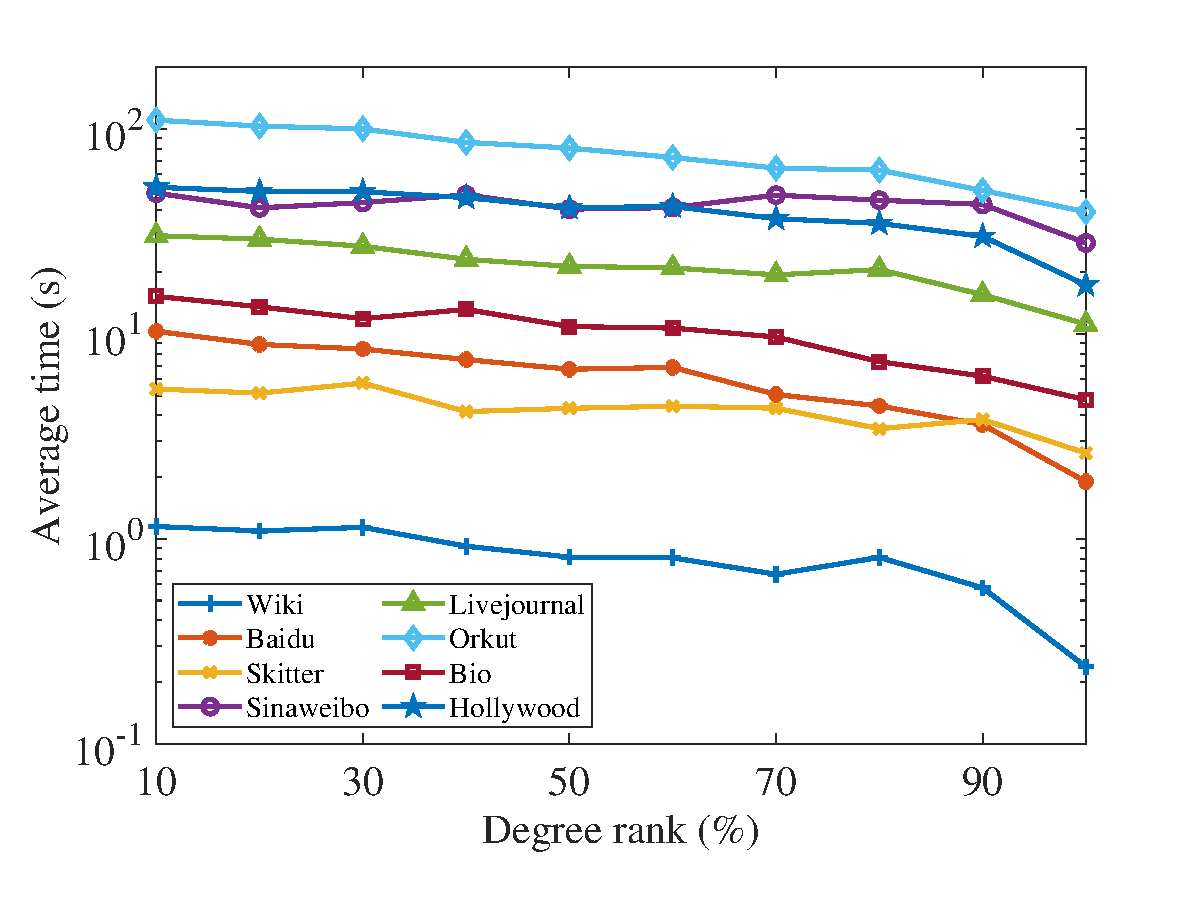
\includegraphics[width=0.18\linewidth]{./figures/path.pdf}}
%\caption{Queries inside communities.}
%\label{fig:inside_query}
%\end{figure}

\subsubsection{K-truss community boundary search.}

\begin{figure}[ht]
    \centering
    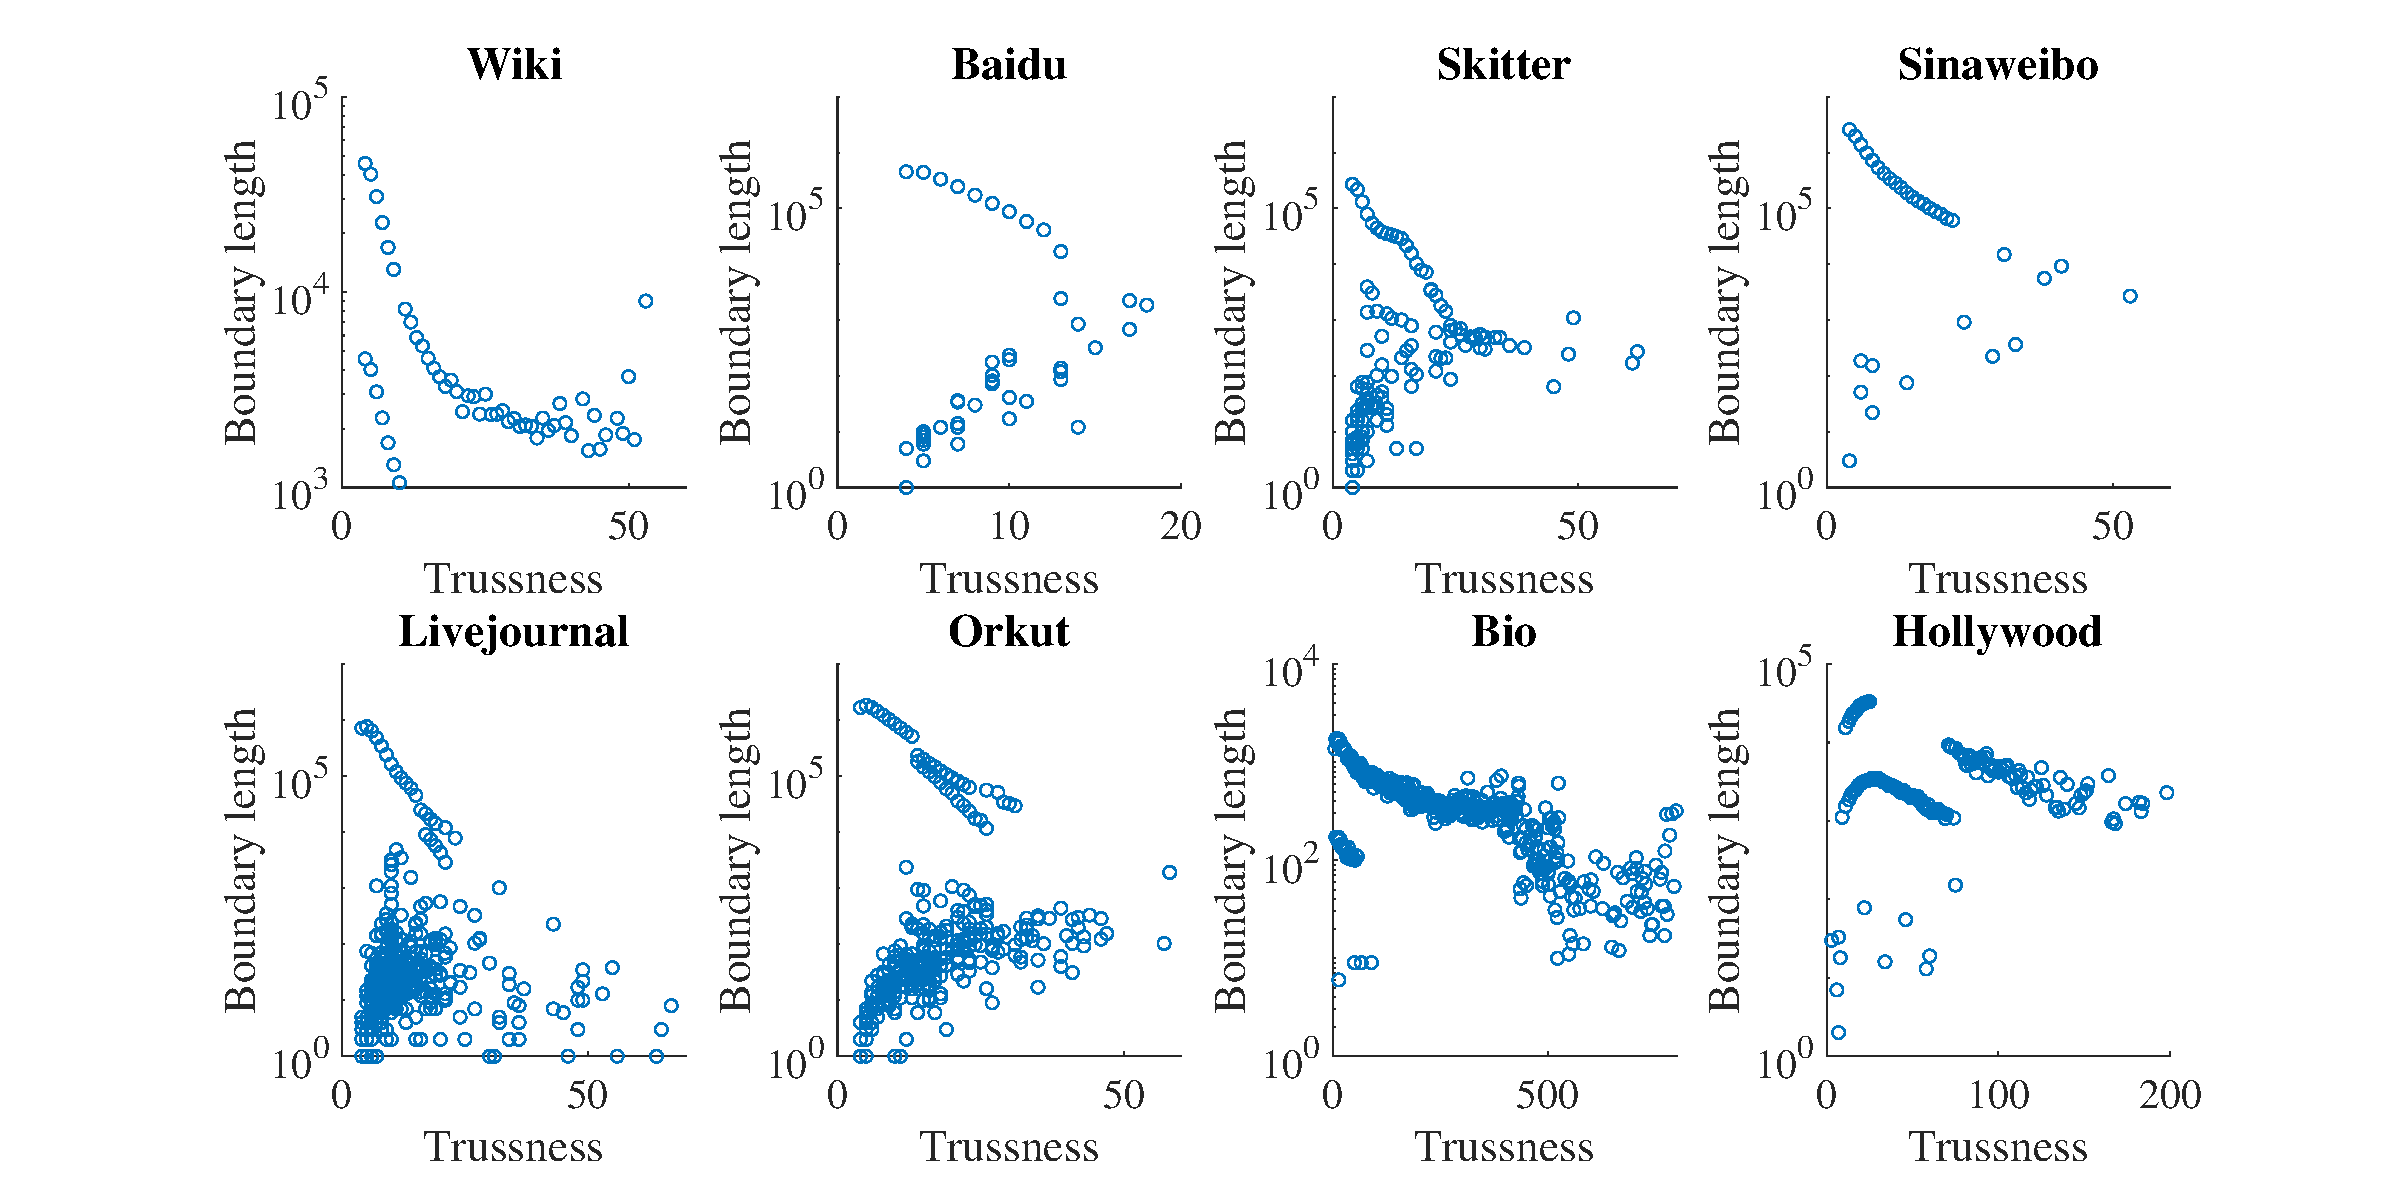
\includegraphics[width=\linewidth]{./figures/boundary_size.pdf}
    \caption{Randomly sampled boundary length for k-truss communities with different trussness.}
    \label{fig:boundary}
\end{figure}

%\vskip 0.1in \noindent \textbf{Boundary search.} 
We randomly select $1000$ query vertices from various degree buckets and perform the boundary search for the k-truss community with highest trussness that contains each query vertex and the trussness of the community and their boundary length in \autoref{fig:boundary}. We can see that in many graphs there is a huge k-truss community of size several magnitude larger than other smaller k-truss communities. This community usually have a hierarchical structure, \ie larger k-truss communities with low trussness contain smaller k-truss communities with high trussness. \autoref{fig:boundary} also shows that the upper bound of the boundary length of k-truss communities decreases as the trussness increases. The main reason for this is that sizes of high trussness k-truss communities are usually smaller than sizes of low trussness k-truss communities. However, the lower bound of the boundary length of k-truss communities increases as the trussness increases. The reason is that there are many small-size k-truss communities which are triangle connected to very few other k-truss communities, \ie they are like isolated islands of the graph and many of them haven't formed a hierarchical structure. 

\subsubsection{Triangle connected maximin path search.}

\begin{figure}[ht]
    \centering
    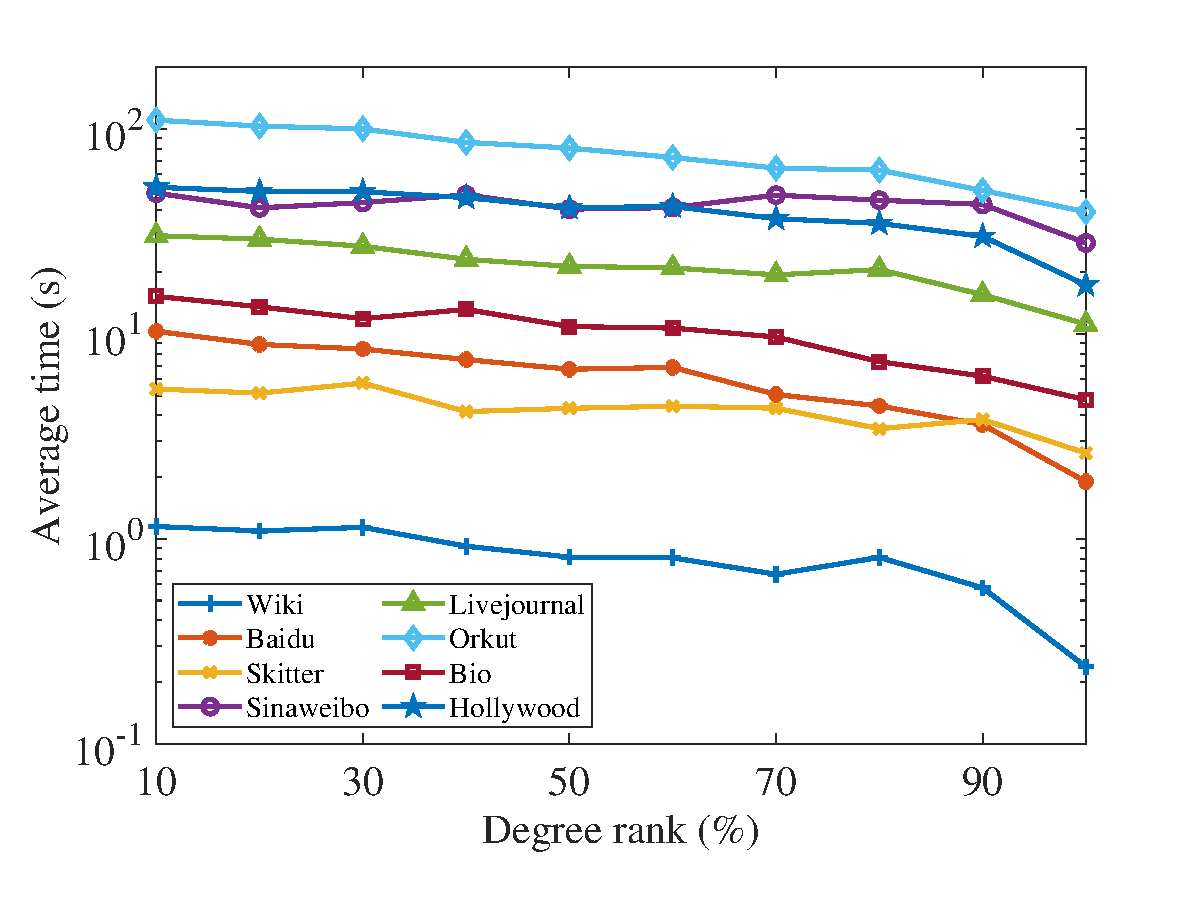
\includegraphics[width=0.5\linewidth]{./figures/path.pdf}
    \caption{Average query time for triangle connected maximim path search.}
    \label{fig:path}
\end{figure}

We randomly select $1000$ pair of vertices from various degree buckets and show the average query time for the triangle connected maximin path search with them in \autoref{fig:path}. 
%\vskip 0.1in \noindent \textbf{Maximin path search.} 
The figure clearly shows that as the degree of vertex increases, the query time decreases. The reason is that for a pair of vertices with high degree, it is more likely that they belong to the same k-truss community with higher trussness and smaller size. So there is no surprise that the query vertices are closer to each other and a triangle connected maximim path between them tends to be shorter. We notice that the triangle connected maximin path search have much higher average query times for the same graph than k-truss community search because it needs to run a BFS traversal inside a target community which is very time-consuming.

\section{Related Works}
\label{relatedwork} 

Our work is most related to the inspiring work~\cite{huang2014querying} which introduce the notion of k-truss community based on triangle connectivity. An index structure call TCP is proposed in~\cite{huang2014querying} that each vertex holds their maximum spanning forest based on edge trussness of their ego-network. Triangle connected k-truss communities mitigate the "free-rider" issue but at the cost of slow computation efficiency especially for vertices belongs to large k-truss communities so that they are not able to meet requirements of queries in some cases. We have use this work as a comparison in section \autoref{evaluation}.

The notion of triangle connected k-truss community is also referred to as $k-(2,3)$ nucleus in~\cite{sariyuce2016fast} where they propose an approach based on disjoint-set forest to speed up the process of nuclues decomposition. We are more emphasize on the fast query process rather speed up the truss decomposition. Also the \treeindex{} is easier to maintain for dynamic graphs.

Our work falls in the category of cohesive subgraph mining~\cite{koujaku2016dense, sozio2010community, cui2014local, li2015influential, cui2013online, mcauley2012learning}, such as clique~\cite{bron1973algorithm, rossi2014fast}, k-core~\cite{cheng2011efficient, shin2016corescope}, k-truss~\cite{huang2014querying, wang2012truss, cohen2008trusses, huang2015approximate, huang2016truss} and quasi-clique~\cite{tsourakakis2013denser}. An $\alpha$-adjacency $\gamma$-quasi-$k$-clique model is introduced by~\cite{cui2014local} for online searching of overlapping communities. $\rho$-dense core is a pseudo clique recently introduced by~\cite{koujaku2016dense} that is able to deliver optimal solution for graph partition problems. The pattern of k-core structures is studied by~\cite{shin2016corescope} for applications such as finding anomalies in real world graphs, approximate degeneracy of large-scale graphs and so on. K-truss decomposition is also studied in~\cite{huang2016truss} for probabilistic graphs.


\section{Conclusion}
\label{conclusion}

In this paper, given an undirected graph G and a set of query nodes $Q$, we formulate a new problem call truss community identity search, which can help answer various query types with multiple query vertices such as max-k truss query, any-k truss query as well as k-truss query. This new proposed problem can be used in many applications as building blocks for community related queries. To solve this problem and k-truss community search efficiently, we propose a 2-level index structure for fast query process. Not only our index structure can support various query types with multiple query vertices. We ourperform state-of-the-art truss index for single vertex k-truss community search. We also develop an efficient algorithm to construct such an index. Extensive experiments on real-world networks show the effectiveness and efficiency of our algorithms. 



\bibliographystyle{ACM-Reference-Format}
\bibliography{reference} 

\end{document}
